\documentclass[11pt, a4paper]{article} % , draft
\usepackage[utf8]{inputenc}

\usepackage{enumitem} % customiçe item dots etc
\usepackage{textgreek} % obv
\usepackage{physics} % for easy derivative notation
\usepackage{amsmath}
\usepackage{amsthm} %theorems
\usepackage{amssymb}
\usepackage{mathtools} % for matrices with blocks inside
\usepackage[scr=boondoxo]{mathalfa}
\usepackage{pst-node}%
\usepackage{mathrsfs}
\DeclareMathAlphabet{\mathpzc}{OT1}{pzc}{m}{it}

\newcommand{\mc}{\multicolumn{1}{c}}
\newcommand{\R}{\mathbb{R}} % command for real R
\newcommand{\Holo}{\mathcal{H}}
\newcommand{\M}{\mathcal{M}}
\newcommand{\C}{\mathbb{C}}
\newcommand{\N}{\mathbb{N}}
\newcommand{\z}{\mathpzc{s}}
\newcommand{\p}{\mathpzc{r}}
\newcommand{\s}{\mathbb{S}}
\newcommand{\W}{\mathbb{W}}
\newcommand{\U}{\mathscr{U}}
\newcommand{\Lg}{\mathscr{L}}
\newcommand{\x}{\mathcal{X}}
\newcommand{\B}{\mathfrak{B}}

\usepackage{csquotes}
\MakeOuterQuote{"}
\setlength{\parskip}{0.3 cm}
\setlength{\parindent}{0 cm}


\usepackage{fancyhdr}

%\usepackage{nath} % authomatic parenthesis stuff
%\delimgrowth=1
\usepackage[left=2cm, right=2cm, top=2.1cm, bottom=2.1cm]{geometry} % set custom margins
\usepackage{graphicx} % to insert figures
\usepackage{grffile}
\graphicspath{{Figures/}} % define the figure folder path
\usepackage{subcaption} % for multiple figures at once each with a caption
\usepackage{multirow} %multirow in tables

\usepackage{caption}
\captionsetup[figure]{font=footnotesize} %adjust caption size
\captionsetup[table]{font=footnotesize} %adjust caption size

\usepackage{booktabs} % for pretty tabs in tables
\usepackage{siunitx} % Required for alignment
\captionsetup{labelfont=bf} % bold face captations

\usepackage{hyperref} % makes every reference a hyperlink
\hypersetup{
    colorlinks=true,
    linkcolor=violet,
    filecolor=[rgb]{0.69, 0.19, 0.38},      
    urlcolor=[rgb]{0.0, 0.81, 0.82},
    citecolor=[rgb]{0.69, 0.19, 0.38}
}

\usepackage{epigraph} % for quotations in teh begginig
\setlength\epigraphwidth{8cm}
\setlength\epigraphrule{0pt}
\usepackage{etoolbox}
\makeatletter
\patchcmd{\epigraph}{\@epitext{#1}}{\itshape\@epitext{#1}}{}{}
\renewcommand{\qedsymbol}{o.\textepsilon.\textdelta}

\newtheorem{prop}{Proposition} %so I can use propositions
\newtheorem{cor}{Corollary} %so I can use corollaries
\newtheorem{defi}{Definition} %so I can use corollaries

\makeatother % all this is for the epigraph
\usepackage{tocloft}

\usepackage{imakeidx} % make index

\makeindex[columns=3, title=Alphabetical Index, intoc]


\title{\vspace{-2cm} {\bf Reality and Causality in the Microscopic World:\\ A Discussion from Quantum Transport Theories}
\vspace{-0.4cm}}
\date{\vspace{-11ex}}
\let\clipbox\relax
\usepackage{adjustbox}
\newcolumntype{?}{!{\vrule width 1.5pt}}
\usepackage{abstract}
\setlength{\absleftindent}{0mm}
\setlength{\absrightindent}{0mm}

\usepackage{tcolorbox}
\DeclareRobustCommand{\mybox}[2][gray!10]{%
\begin{tcolorbox}[   %% Adjust the following parameters at will.
        left=0.2cm,
        right=0.2cm,
        top=0.15cm,
        bottom=0.15cm,
        colback=#1,
        colframe=#1,
        width=\dimexpr\textwidth\relax, 
        enlarge left by=0mm,
        boxsep=5pt,
        arc=0pt,outer arc=0pt,
        ]
        #2
\end{tcolorbox}
}

\usepackage{anyfontsize}
\newenvironment{kapituloBerria}[1][]
  {\clearpage           % we want a new page          %% I commented this
   \thispagestyle{empty}% no header and footer
   \vspace*{\stretch{2}}% some space at the top
   \raggedleft          % flush to the right margin
   {\textbf{{\fontsize{60}{40}\selectfont \hspace{+9.5cm}#1\newline \newline}}}
   \bf
   \fontsize{30}{20}\selectfont
  }
  {\par % end the paragraph
   \vspace{\stretch{3}} % space at bottom is three times that at the top
   \clearpage           % finish off the page
  }

\usepackage{listings}
\usepackage{xcolor}
\lstset{language=C++,
                basicstyle=\ttfamily,
                keywordstyle=\color{blue}\ttfamily,
                stringstyle=\color{red}\ttfamily,
                commentstyle=\color{green}\ttfamily,
                morecomment=[l][\color{magenta}]{\#}
    backgroundcolor=\color{black!5}, % set backgroundcolor
    basicstyle=\footnotesize,% basic font setting
}
%\DeclareMathSizes{display size}{text size}{script size}{scriptscript size}.
\DeclareMathSizes{10}{10}{10}{10}
\setlength{\footnotesep}{0.55\baselineskip}
\begin{document}
\pagenumbering{gobble}



%\maketitle

%%{\bf Chapter on {\em “Physics and the Nature of Reality: Essays in Memory of Detlef Dürr”.}}
%%
%%\begin{center}
%%{\bf Abstract }
%%\end{center}
%%Paraphrasing Feynmann, perhaps, the main reason why the so-called Copenhagen (or orthodox) quantum theory is so popular among the physicists and engineers is because “I can safely say that nobody understands [it]”. Many physicists and engineers take profit of the mathematical machinery of the Copenhagen theory without paying attention to its ontology, which implies that a quantum object has no microscopic properties (unless a property is measured, or the quantum object is an eigenstate of some property). Such an orthodox view of a microscopic world, empty of properties, is specially unsuitable to understand and to develop approaches to predict modern nanoelectronics, as we discuss along this chapter. As an alternative, physicists dealing with the foundations of quantum transport and open systems have developed different approaches in terms of some type of causal motion of electrons. When dealing with nanodevices, the Copenhagen ontology affirms that electrons are nowhere since their positions are undefined until measured, while causal motion approaches say that electrons can be perfectly understood as particles traversing a device with well-defined positions, independently of the measurement. This last view certainly holds true for treatments based on the Bohmian theory. Even for quantum phenomena of light, such as spontaneous emission or photon partition noise, the Bohmian theory allows an explanation from well-defined electromagnetic fields interacting with electrons, which is contrary to the standard Copenhagen approach. The above examples, developed in this chapter, emphasize that the main merit of the Bohmian theory is eliminating the observer/measurement as the “creator” of the microscopic reality, showing that a well-defined description at all times, of the microscopic properties of a quantum system, is available (where particles are particles and fields are fields at all times). Such a microscopic description does not only provide conceptual advantages, but also important numerical ones when electron devices are understood, in general, as non-Markovian open quantum systems.   

\newpage
\pagenumbering{arabic}
\setcounter{page}{1}
\begin{center}
\section*{ Bohmian Mechanics as a Practical Tool \vspace{0.2cm}\vspace{0.1cm}\\ \small Xabier Oyanguren\footnote{\em Departament de Física, Universitat Autònoma de Barcelona, 08193 Bellaterra, Barcelona, Spain}, Carlos F. Destefani\footnote{\em Departament d’Enginyeria Electrònica, Universitat Autònoma de Barcelona, 08193 Bellaterra, Barcelona, Spain}, Matteo Villani$^2$, David K. Ferry\footnote{\em School of Electrical, Computer, and Energy Engineering, Arizona State University, Tempe,
AZ 85287 USA} and Xavier Oriols$^2$}
%\vspace{0.2cm} \small when tools harnessing beyond-observable notions happen to be Bohmian in disguise }
\vspace{-0.5cm}
{\bf \small - Chapter on {\em “Physics and the Nature of Reality: Essays in Memory of Detlef Dürr” - }}\vspace{-0.32cm}
\end{center}

\hspace*{4mm} Questioning whether "there are" electrons inside our mobile phones sounds like an absurd reflection, and yet the orthodox (also called Copenhagen or standard) quantum theory is not able to affirm it. Under this theory, a quantum object has a well-defined property (like the position) only when its wavefunction is an eigenstate of the associated operator. We know that this happens when the property is "strongly measured". But in general, the wavefunction is in a superposition of eigenstates for the operator of that observable, meaning nothing can be said about it: the property becomes "unspeakable" while not measured. Consequently, the standard theory states that it is meaningless to talk about say, the positions of the electrons inside the active regions of nanoscale devices, because while in operation, their position is never (strongly) measured. Thus, there is no chance for an affirmative answer to our initial question. And yet, consciously or not, no engineer or applied physicist can seriously accept there is no electron in an operating nano-device like a transistor \cite{where}. Fortunately, there are alternative interpretations by which electrons have a position irrespective of their measurement and the state of superposition of their wavefunction, e.g., the well known Bohmian theory \cite{Bohm,Holland, Durr,JordiXavier}. \vspace{-0.07cm} 

What might be more relevant from a practical point of view however, is that even if one turns a blind eye to these "picky unspeakabilities" of the orthodox theory, their implications also limit the employable practical tool-set. Under this restricted vocabulary, the modeling of some scenarios looks unnecessarily pathological, leaving tied the hands of the orthodox, in addition to their words. Example of such {\bf practical} limitations of the orthodox theory are the search of measurement operators in some scenarios (like the multi-electron displacement current \cite{equiv, Pel}), or the "cumbersome" demand of some measurement devices to be modeled as non-Markovian environments of the studied systems \cite{Thz}. As ironic as it is, the orthodox that even still look for tools that allow the prediction of the phenomenological manifestations of such “pathological” scenarios (to predict the expectation or correlation of dynamical variables or predict the reduced density
of non-Markovian open quantum systems),  "accidentally" reach concepts like position post-selected weak values or the conditional wavefunction, which are Bohmian in disguise, as we will explain \cite{interpretSSE,NMisModal}.\vspace{-0.1cm}

In this chapter, we will take a trip around several hot-spots where Bohmian mechanics and its capacity to describe the microscopic reality even in the absence of measurements, can be harnessed as computational tools, in order to help in the prediction of phenomenologically accessible information (equally useful for the followers of the orthodox theory). %We will then justify how the additional step to assume an ontological interpretation for such pragmatic tools, turns out to be practically useful, even when one is only interested in computational (and not foundational) issues.

We can easily arrive to these conclusions through the concepts of conditional wave-function (CWF) and effective wave-function (EWF), introduced by {\em Dürr et al.} in Ref. \cite{Absolute}, together with the understanding of the measurement dilemma they enlighten. We will therefore review them in the first section, along with how the density matrix formalism and any general quantum operation can be understood in Bohmian terms. All this will lead us in a natural way to the main theses of the chapter. For instance in section two, we will show how a Stochastic Schrödinger Equation (SSE), used to compute the reduced density matrix of a non-Markovian open quantum system, necessarily seems to employ CWF-s. We will see that by dressing these CWF-s with an interpretation, the Bohmian theory can prove to be a useful tool in the search for SSE-s. In section three, we will introduce how an orthodox observable can be computed from Bohmian trajectories, as if it was a feature emerging from them, arriving to be able to derive the observable operator itself from Bohmian mechanics. With this conception, since the trajectory of an "unmeasured" system is well-defined at all times in Bohmian mechanics, we will be free to speak about their properties (even if only some of them $-$ or none of them $-$ are given an ontological status). Moreover, not only will we be able to simulate and talk about them, but we will see that they can be experimentally determined. This will bring about several practical applications.


\subsection*{1. Introduction: A Suggestive Review}
\vspace{-0.2cm}

Before going into the details, note that along the whole chapter, we will only discuss basic {\bf non-relativistic quantum phenomena}. The spirit is to show that for this kind of phenomena and their formulation, the Bohmian theory provides a most convenient narrative. Yet, it is of course possible if not certain, that a deeper level in the quantum theory may require other frameworks.\vspace{-0.3cm}

\subsubsection*{1.1. The Conditional and Effective Wavefunctions}
\vspace{-0.2cm}

Given a quantum system of $N$ degrees of freedom described by the real coordinate vector $\vec{q}=(q_1,..., q_n)\in\Omega_t\subseteq\R^N$, we can describe its time-evolution with the use of a complex wavefunction $\Psi(\vec{q},t)=\rho^{1/2}(\vec{q},t)e^{i\mathcal{S}(\vec{q},t)/\hbar}$ (encoding the two real fields $\mathcal{S}$ and $\rho$), and an associated Bohmian trajectory $\vec{q}^{\:\xi}(t)\equiv \vec{q}\:(\vec{\xi},t)$, the initial condition of which is given by the label space vector $\vec{\xi}\in\Omega_0\subseteq\R^N$, such that $\vec{q}^{\:\xi}(t=0)=\vec{\xi}$. This trajectory is guided by the wavefunction through the "guidance law"
\begin{equation}\label{GL}
\dv{q_k^{ (\xi)}(t)}{t} = v_k(\vec{q},t)\Big\rvert_{\vec{X}=\vec{q}^{\:\xi}(t)}:=\frac{1}{m_k} \pdv{\mathcal{S}(\vec{q},t)}{x_k}\Big\rvert_{\vec{q}=\vec{q}^{\:\xi}(t)}
\end{equation}
while the wavefunction itself is guided by the Schrödinger Equation \cite{Bohm,Holland,Durr,JordiXavier}
\begin{equation}\label{SE}
i\hbar\pdv{\Psi(\vec{q},t)}{t}=\Big[ \sum_{k=1}^N \frac{\hbar^2}{2m_k}\pdv[2]{}{q_k}+U(\vec{q})\Big]\Psi(\vec{q},t)
\end{equation}
where $m_k$ is the mass associated with the $k$-th degree of freedom, $v_k$ is the velocity field piloting the $k$-th degree of the Bohmian trajectories and $U$ denotes the potential describing the interaction between the degrees of freedom (since we consider an isolated system we assume no time dependence on $U$). The most general isolated system we could consider is the whole Universe, where $\vec{q}$ would reflect its degrees of freedom or {\bf configuration}. The fact that a single trajectory $\vec{q}^{\:\xi}(t)$ is assigned to the whole Universe shows the deterministic nature of the Bohmian theory (at least, at the ontological level). 

Let us now partition the whole Universe in a subsystem of interest S, of $n<N$ degrees of freedom $\vec{x}=(x_1,...,x_n)$, and its environment, of degrees of freedom $\vec{y}=(y_{n+1},...,y_N)$; where we identify $\vec{q}\equiv (\vec{x},\vec{y})$. We could associate one wavefunction to the system and one to the environment, both labeled by the initial joint configuration $\vec{\xi}$, as $\psi^\xi(\vec{x},t):=\Psi(\vec{x},\vec{y}^{\:\xi}(t),t)$ and $\phi^\xi(\vec{y},t):=\Psi(\vec{x}^{\:\xi}(t),\vec{y},t)$. These are particular cases of the so called {\bf conditional wavefunctions} (CWF-s). In general, a CWF is a slice of a wavefunction, obtained by evaluating some of its degrees of freedom along a (Bohmian) trajectory, while leaving the rest un-evaluated \cite{Absolute, JordiXavier}. 

As proved in \cite{GJ}, the full Schrödinger Equation \eqref{SE}, ruling the dynamics of the whole, can be re-written exactly into two coupled dynamical sets of equations ruling the motion of the two presented CWF-s. Assuming we can write $U(\vec{x},\vec{y}\,)=U_x(\vec{x}\,)+U_{xy}(\vec{x},\vec{y}\,)$, for the system we have\footnote{For the environment they will be the same but changing the CWF and the index ranges.}:\vspace{-0.2cm}
\begin{equation}\label{SE.GJ}
i \hbar \pdv{\psi^\xi (\vec{x},t)}{t} = \qty[\sum_{k=1}^n\frac{\hbar^2}{2m_k} \pdv[2]{}{x_k} + U_x(\vec{x}\,)+ U_{xy}(\vec{x}, \vec{y}^{\: \xi}(t)) + G(\vec{x}, \vec{y}^{\: \xi}(t),t)+i\ J(\vec{x}, \vec{y}^{\: \xi}(t),t)] \psi^\xi (\vec{x},t)
\end{equation}
with $G$ and $J$ the real and complex parts of the so called {\bf quantum correlation potential}:
\begin{equation}\label{G.Bohm}
G(\vec{x},\vec{y}^{\:\xi}(t),t):=\sum_{j=n+1}^N\qty[-\frac{1}{2}m_j\qty(v_j(\vec{x},\vec{y}^{\: \xi}(t),t))^2-\frac{\hbar^2}{2m_j\rho^{1/2}(\vec{x},\vec{y}^{\:\xi}(t),t)}\qty(\pdv[2]{\rho^{1/2}(\vec{x},\vec{y},t)}{y_j})\Big\rvert_{\vec{y}=\vec{y}^{\:\xi}(t)} ]\vspace{-0.2cm}
\end{equation}
\begin{equation}\label{J.Bohm}
J(\vec{x},\vec{y}^{\:\xi}(t),t):=-\frac{\hbar}{2}\sum_{j=n+1}^N\pdv{}{y_j}v_j(\vec{x},\vec{y},t)\Big\rvert_{\vec{y}^{\, \xi}(t)}
\end{equation}
where we recognize as $G$ the difference between the quantum potential \cite{JordiXavier, Durr} and the kinetic energies of the trajectory of the environment; and as $J$, the spatial variation in the environment axes $y_j$ of their associated Bohmian velocity\footnote{Note that while multiple stacked CWF-s for the subsystem around $\vec{y}^{\:\xi}(t)$ are required to compute $G$ and $J$, the guidance for the trajectory of the subsystem $\vec{x}^{\:\xi}(t)$, is given entirely by the CWF at $\vec{y}^{\:\xi}(t)$: denoting $\psi^\xi (\vec{x},t)=r^\xi(\vec{x},t)e^{is^\xi(\vec{x},t)/\hbar}$, then $\dv{}{t}x_k^{(\xi)}(t)=\frac{1}{m_k}\pdv{s^\xi(\vec{x},t)}{x_k}\big\rvert_{\vec{x}=\vec{x}^{\:\xi}(t)}$ for $k\in\{1,...,n\}$.}. The evaluation of both $G$ and $J$, involve at each $\vec{x}$, a derivative of the phase $\mathcal{S}$ or the magnitude $\rho$ of the full wavefunction $\Psi$ along the environment coordinates $\vec{y}$, centered at the trajectory position $\vec{y}^{\:\xi}(t)$. This means they require information of the wave function (the CWF-s) over nearby possible trajectories $\vec{y}^{\:\xi'}(t)=\vec{y}^{\:\xi}(t)+\Delta \vec y$, with $|\Delta\vec y\, |\rightarrow 0$. The peculiarity of having the dynamics of a single CWF linked to the dynamics of other CWF-s is known as the quantum wholeness \cite{JordiXavier}, and it lays in the heart of the discussion about Markovianity, as we will see.

Now, we might ask when the subsystem CWF $\psi^\xi(\vec{x},t)$ behaves as if it was an independent closed quantum system wavefunction, ruled by a unitary Schrödinger Equation \eqref{SE}. This happens only while both $G$ and $J$ vanish and $U_{xy}(\vec{x},\vec{y}^{\,\xi}(t))\simeq V(\vec{x},t)$ with a same shape irrespective of the trajectory $\vec{\xi}$.\footnote{ If only $J$ vanished, the CWF would already seem to be ruled by a unitary Schrödinger Equation of a closed system, with a real potential: $V(\vec{x},t):=U(\vec{x},\vec{y}^{\:\xi}(t))+G(\vec{x},\vec{y}^{\:\xi}(t),t)$. Yet, computationally, a quantum description for the environment in order to evaluate $G$ and the trajectory $\vec{y}^\xi(t)$ would still be required, making it not independent of the environment's evolution. } Whenever this is the case, we can say that the CWF of the system is its {\bf effective wavefunction} (EWF). The question is then: when do these three happen? One of the most important cases is just after a strong measurement of the subsystem. 

\vspace{-0.2cm}

\subsubsection*{1.2. The orthodox collapse law in the Bohmian theory}
\vspace{-0.1cm}

We are routinely interested in subsystems much smaller than the whole Universe. In many circumstances, such subsystems can reasonably be assumed to be modelable effectively as closed systems described by an EWF $\psi(\vec{x},t)$. It is also reasonable to assume that similar subsystems can be prepared in other places and times, each of them described by the same wavefunction $\psi(\vec{x},t)$. We cannot predict with certainty the trajectory $\vec{x}^{\:\xi}(t)$ of each copy (unless we measured it, and then spoiled its wavefunction, making them be no longer copies), but by the Quantum Equilibrium principle, proved in Ref. \cite{Absolute}, if the trajectory of the whole Universe had a "typical" initial condition $\vec{\xi}$, the probability density of the position $\vec{x}^{\:\xi}(t)$ at the $t$-th time of any of the experiments will be given by $|\psi(\vec{x},t)|^2$. The point is that to measure a property of these subsystems, we need to open them temporarily to allow their interaction with a measurement apparatus that will convey the information to us. The orthodox theory explains the effect of this interaction by postulating a non-unitary "collapse law". The Bohmian theory can explain its effect using only the unitary evolution \eqref{SE}, as we exemplify now.%If understood as a physical process, this may lead to confusion. Yet, as von Neumann himself in his seminal book \cite{vonNeumann} explains \cite{NeumannNoCollapse}, it is better to understand it as an effective process that may be placed at an arbitrary point between the subsystem and the macroscopic device. Interestingly, Bohr himself did not either believe in a physical collapse and instead owned it to the contextuality of experimental protocols \cite{Dirac} in terms of macroscopic devices \cite{Bohr}. Both beliefs are naturally satisfied by the Bohmian description of the measurement, which does not need to postulate any collapse law, as we exemplify now with the discrete spectrum observable case.

Given the closed quantum system S with EWF $\psi(\vec{x},t)$, to take a strong measurement of the property $B$, as suggested by von Neumann \cite{vonNeumann} and explained in terms of Bohmian mechanics in Refs. \cite{Durr, JordiXavier, Holland}, we have to consider the degrees of freedom of a macroscopic measuring apparatus, $z\equiv y_{n+1}$, called the pointer, as part of the environment of S. It will be a good apparatus if its pointer has a position at the initial time $t=0$, $\vec{z}^{\;\xi}(0)$, close to its rest position, independently of the rest of the environment, meaning it has an EWF similar to $\varphi(z,0)=c e^{-z^2/4\sigma^2}$, or in ket notation $\ket{\varphi(t)}_M=\int\varphi(z,0) \ket{z}dz$, with $c=1/((2\sigma\pi)^{1/4})$ a normalization constant and $\sigma$ small. Then, for the apparatus to extract information of the subsystem S, they are made to interact for a time $T$ through the von Neumann Hamiltonian $\hat{H}_{MS}=\bar{\mu}(t)\,\hat{p}_M\otimes \hat{B}_S$, where $\hat{p}_M$ is the momentum operator of the dial and $\hat{B}_S$ is the operator related with the property $B$ of the system we wish to measure. This is the Hamiltonian that provokes the position of the pointer to get entangled with the possible eigenstates of $B$. Note the measurement strength is defined as $\mu:=\int_0^T\bar{\mu}(t)dt$. Now, if the observable $B$ has countable spectrum, such that $\hat{B}_S=\sum_k b_k \ket{b_k}_S\bra{b_k}_S$, with $\{\ket{b_k}_S\}_k$ an orthonormal basis of S and $\ket{\psi(0)}_S=\sum_k \beta_k(0)\ket{b_k}_S$ with $\beta_k(0)=\bra{b_k}_S\ket{\psi(0)}_S$, the Schrödinger equation \eqref{SE} causes a unitary evolution $\hat{U} \null_{0}^T=e^{-i\mu T \hat{H}_{MS}/\hbar}$ of the composed initial state $\ket{\Phi(0)}_{MS}=\ket{\varphi(0)}_M\otimes\ket{\psi(0)}_S$ as:\vspace{-0.15cm}
\begin{equation}\label{postM1}
\ket{\Phi(0)}_{MS} \overset{\hat{U}_{0}^T}{\longrightarrow} \ket{\Phi(T)}_{MS}=\sum_k \beta_k(0)\qty(\int c \; e^{-\frac{(z-b_k\mu T)^2}{4\sigma^2}}\ket{z}_M dz )\otimes \ket{b_k}_S \vspace{-0.15cm}
\end{equation}
This means that the probability density for the Bohmian position of the dial $z^\xi(T)$ is concentrated in $z$, in several Gaussians of weights $|\beta_k(0)|^2$. Each $k$-th Gaussian is centered in a different $z=b_k \mu T$. The interaction strength $\mu$ must be big for the dial to determine a single result. That is because this way the Gaussians can have a disjoint support, meaning that around each Gaussian, the CWF for the system S is always proportional to one of the eigenstates $\ket{b_k}_S$, linked to a single associated eigenvalue $b_k$ of $B$ (indicated by the dial). Then by the eigenstate-eigenvalue link, the standard theory allows us to say that the property $B$ of S has the value $b_k$. At this point, the orthodox suddenly say the subsystem wavefunction "collapses" into the $\ket{b_k}_S$ closest to the dial's position $z^\xi(0)$ \cite{vonNeumann}. The observation introduced by the Bohmian is that these Gaussians modulating different CWF-s must be {\bf macroscopically disjoint} in $z$, since only this way the dial can macroscopically show the different measurements. This makes the correlation potentials $G,J$ of Eqs. \eqref{G.Bohm}, \eqref{J.Bohm}, between the dial M and the syubsystem S vanish. Importantly, since any interaction between M and S is set off for significant times $t>T$, the potential energy will get factored as $U(\vec{x},z)=U_x(\vec{x})+U_z(z)$. In consequence, the macroscopic separation of the other CWF-s (the "empty waves") will only get more disjoint \cite{Absolute}, making $G$,$J$ still non-zero at any significant future time. This means, the CWF for S can be evolved for $t>T$, as if it was again an independent closed quantum system wavefunction: it is an EWF. From the perspective of S, omitting $t\in(0,T)$, it will have looked like the state $\ket{\psi}$ suffered a "collapse" into $\ket{b}_k$, with probability $|\beta_k(0)|^2$.


Notice that, either the assumption that for time $t>T$, M does not interact anymore with S, or that the environment entanglement with S is lost by some sort of thermalisation (by which the empty waves $-$ the rest of CWF-s that are not sliced at $z=z^{\:(\xi)}(T)$ $-$ get macroscopically dispersed), mean that the information of the subsystem that was "leaked" to the environment M: the "empty waves" themselves, do not interact back with the EWF of S. Any of these two assumptions thus imply that the environment effectively "forgets" the entanglement achieved with S. This is an environment behavior we could call memory-less or Markovian.%\footnote{The evolution of macroscopically disjoint CWF-s in configuration space rapidly makes them even more disjoint \cite{Absolute}. Thus, such an assumption is reasonable in many scenarios even if the same measuring apparatus is repeatedly used.}\vspace{-0.1cm}

As a consequence, since the description of the environment M will only be useful for the measurement time interval $(0,T)$, and can then be discarded, we can instead explain the apparent projection of the state of the subsystem into an eigenstate of the operator B, $\ket{\psi(t)}\to \ket{b_k}_S$, with a set of effective-"collapse" orthogonal projectors $\{\hat{\Pi}_k\}_k$ (with $\hat{\Pi}_k=\ket{b_k}_S\bra{b_k}_S$), without the need to explicitly formalize M and the whole interaction process \cite{Durr}. We shall not forget however that this is just a short-cut in the modeling.\vspace{-0.3cm}



\subsubsection*{1.3. How to use the Effective Collapse for a more general Measurement}\vspace{-0.1cm}

Notice that the effective-"collapse" described above need not be part of a measurement by an observer. It could also happen as the effect of a more general environment coupling. This implies that if part of the environment gets entangled with S and this environment portion then suffers an effective collapse as the one in the strong measurement, S will also seem to suffer an effective-"collapse", but now into non-necessarily orthogonal nor linearly-independent states (nor a number of states limited by the dimensionality of the Hilbert space of S). It will seem to suffer a non-unitary non-orthogonal projection. If the effective collapse of the enviornment was caused by its strong measurement, giving information to an observer, this is called a {\bf generalized measurement} \cite{Generalized, Durr}. 

Given the initial state $\ket{\psi}_S$ of S, and a fiducial state $\ket{\theta}_A$ for an ancilla A, using an entangling unitary $\hat{U}_{AS}$, we get: $\hat{U}_{AS}\ket{\theta}_A\otimes\ket{\psi}_S=\sum_m \ket{m}_A\otimes \ket{\psi_m}_S$, where $\ket{\psi_m}_S:=\bra{m}_A\otimes\hat{I}_S \big(\hat{U}_{AS}\ket{\theta}_A\otimes\ket{\psi}_S\big)$ is an unnormalized S state called the $m$-th {\bf conditional state} of S, which is entangled with the state $\ket{m}_A$ of A. If we now perform a strong measurement on A for the orthonormal $\{\ket{m}_A\}_m$ basis (coupling a dial M to A and branching A in EWF-s consisting of the measured eigenstates), ancilla-subsystem EFW-s proportional to $\ket{m}_A\otimes \ket{\psi_m}_S$ would be generated as a function of the Bohmian position of the dial M\footnote{Note that the conditional state $\ket{\psi_m}_S$ is in fact a subsystem CWF, obtained by evaluating the dial position of M indicating the state $\ket{m}_A$ (for any trajectory position of A) in the composite wavefunction.}. By the Quantum Equilibrium principle \cite{Absolute}, the $m$-th result would be observed with a probability equal to the norm squared of its conditional state $P_m:=|\bra{\psi_m}_S\ket{\psi_m}_S|^2$. If we then set-off the interaction between A and S for all future times, the subsystem S will have seemed to "collapse" into the EWF $\ket{\psi_m}_S/\sqrt{P_m}$ with probability $P_m$, since it will now evolve independently of $A$ (we assume again $A$ is an environment for the subsystem S with a Markovian behavior). %Now, these conditional states $\ket{\psi_m}_S$ need not even be linearly independent.

Consequently, as with the projective measurement of S, we can shortcut the formalization of A and its measurement, by just considering a set of general measurement (linear) operators on S (called POVM-s) $\big\{\hat{\Omega}_m:=\bra{m}\otimes\hat{I}_S\:\hat{U}_{AS}\ket{\theta}_A\otimes\big\}_m$, sending S states to post-measurement (unnormalized) EWF-s as: $\hat{\Omega}_m\ket{\psi}_S$. The only requirement for them is: $\sum_m \hat{\Omega}_m^\dagger\hat{\Omega}_m=\hat{I}_S$, so that the $m$-probabilities add-up to one. This is satisfied because $\hat{\Omega}_m\ket{\psi}_S=\ket{\psi_m}_S$ is the (unnormalized) post-measurement EWF of S, the squared norm of which is the probability $P_m$ to observe $m$ and thus get the EWF $\ket{\phi_m}_S:=\ket{\psi_m}_S/\sqrt{P_m}$ for S \cite{Generalized, Durr}. The reason why such an A and $\hat{U}_{AS}$  exist for {\bf any} set of linear operators $\{\hat{\Omega}_m\}_m$ satisfying the stated restriction, will be seen in a moment. Note that, the orthogonal projectors $\hat{\Pi}_k$ of the strong measurement are naturally a subclass of generalized measurement POVM-s.\vspace{-0.15cm}

\subsubsection*{1.4. The Density Matrix in this Bohmian Narrative}\vspace{-0.15cm}
Let us now motivate the \textbf{density matrix} formalism from our Bohmian perspective. Consider the state $\ket{\psi(0)}$ and the measurement POVM-s $\{\hat{\Omega}_m\}_m$ for a measurement taking a time $T$, that leave $\ket{\psi(0)}$ in the possible EWF-s $\ket{\phi_m(T)}:=\hat{\Omega}_m\ket{\psi(0)}/\sqrt{P_m}$, with associated probabilities $P_m:=\bra{\psi(0)}\hat{\Omega}_m^\dagger \hat{\Omega}_m\ket{\psi(0)}$. If we were not interested in a particular outcome, but we wanted to keep track of all possible post-measurement EWF-s from time $T$ to $t>T$, we could first organize them in a set of vector-probability pairs $\Lambda_{T}:=\{\big(\ket{\phi_m(T)},\ P_m\big)\}_m$, and unitarily evolve its wave-vectors with say, $\hat{U}_{T}^{t}$, such that $\Lambda_{t}:=\big\{\big(\hat{U}^t_T\ket{\phi_m(T)},\ P_k\big)\}_k=\{\big(\ket{\phi_m(t)},\ P_m\big)\}_k$. Now, if a second measurement happened, taking time $T'$, with effective operators $\{\hat{\Omega}'_j\}_j$, we would need to branch each of the independent states in $\Lambda_t$ into the corresponding projected states and update their probabilities: $\Lambda_{t+T'}:=\big\{ \big(\hat{\Omega}_j'\ket{\phi_m(t)}/\sqrt{P_{(j|m)}},\ P_kP_{(j|m)}\big)\big\}_{m,j}$ with $P_{(j|m)}:=\bra{\phi_m(t)}\hat{\Omega}^{'\dagger}_j\hat{\Omega}_j\ket{\phi_m(t)}$ the probability to get the $j$-th outcome if we obtained the $m$-th one before. Importantly, the operator $\hat{\Omega}'_j$ could happen to send any state to the same space, if for example $\hat{\Omega}'_j=\ket{\varphi_j}\bra{\varphi_j}$. In consequence, the normalized state $\hat{\Omega}'_j \ket{\phi_m}/\sqrt{P_{(j|m)}}$ would be the same state $\ket{\varphi_j}$ for all $m$, and we would need to unify them in our $\Lambda_{t+T'}$ set, updating the probability for this state with the contributions of all the cases that lead to it: $P_{(j|\cdot)}:=\sum_m P_mP_{(j|m)}$. But this is quite cumbersome. It is true that to have a full Bohmian description, we should keep track of the possible Bohmian trajectories for each wave-vector. However, if we could afford the loss of ontological detail (as do the orthodox) and just cared for phenomenological probabilistic predictions like $P_m$ or $P_{(j|\cdot)}$, there is a convenient structure that works "automatically" as our sets $\Lambda_t$. This is a "matrix" operating on wave-vectors in which we set the possible EWF-s as its composing ket-bra-s, with the probability of each EWF as coefficient. This positive-definite matrix used as "posible state-probability" pair container is called a {\bf "density matrix"} \cite{vonNeumann, Durr, Holland}. 

It is trivial to see that it works as we wanted for post-measurement states. For example, in order to get the post-measurement density matrix for the first measurement, $\hat{\rho}(T) = \sum_m P_m\ket{\phi_m(T)}\bra{\phi_m(T)}$, we can just take the matrix for the initial state $\hat{\rho}(0):=\ket{\psi(0)}\bra{\psi(0)}$, and compute $\hat{\rho}(T)=\sum_m \hat{\Omega}_m^\dagger\hat{\rho}(0)\hat{\Omega}_m$. Then, if we apply a unitary evolution $\hat{U_T^t}$ (or in fact any linear operator) at each side of the matrix (the Hermitian conjugate in the left), we will be applying the operator to each state-vector inside it, "independently of the rest": $\hat{\rho}(t)=\hat{U}_T^{t\,\dagger}\hat{\rho}(T)\hat{U}_T^{t}=\sum_m P_m\ket{\phi_m(t)}\bra{\phi_k(t)}$. Just as we wanted. Then, for the second measurement we repeat the trick and now the same states $\ket{\varphi_j}$ will automatically be gathered in a single ket-bra. Not only the time evolution and successive effective-collapses are easily managed with such a structure, but single time measurement probabilities for an arbitrary operator $\hat{\Omega}_\alpha$ are easily computed as: $P(\alpha)=tr[\hat{\Omega}_\alpha^\dagger \hat{\Omega}_\alpha\hat{\rho}]$, where $tr$ is the trace operation.

Although very useful for ensemble single-time statistical predictions in effective collapse scenarios, a Bohmian should always keep in mind that the microscopic detail of what is happening is lost when using these density matrices, both regarding the Bohmian trajectory and the state-vectors themselves (since different vector-probability sets yield the same matrix). Importantly, the state-vector and the trajectory of the Universe are still the essential state descriptors in the Bohmian theory, because the Universe as a whole should be described by a determined state-vector.

The so called "partial trace" operation is tigthly related to these post-measurement density matrices. If the density matrix of an ancilla-subsystem composite is $\hat{\rho}_{AS}$, given an arbitrary orthonormal base of A, $\{\ket{m}_A\}_m$, the partial trace of $\hat{\rho}_{AS}$ over A is defined as: $tr_{A}[\hat{\rho}_{AS}] := \sum_k \bra{m}\otimes \hat{I}_S(\hat{\rho}_{AS})\ket{m}\otimes \hat{I}_S$ \cite{Generalized, Durr}. We call the result, the {\bf reduced density matrix} of S. Its relation with measurements is the following one. The partial trace of M on the composite pure state $\hat{\rho}_{MS}(T)=\ket{\Phi(T)}_{MS}\bra{\Phi(T)}_{MS}$ describing the post-measurement state of Eq. \eqref{postM1}, under the effective "collapse" conditions for $\mu,T,\sigma$, precisely yields for the subsystem S, the unconditional post-measaurement density matrix made by the possible "collapsed" EWF-s $\rho(T)_S=\sum_k |\beta_k|^2\ket{b_k}_S\bra{b_k}_S$. The same happens in any generalized measurement: the partial trace of A in the state $\hat{U}_{AS}\ket{\theta}_A\otimes\ket{\psi}_S$ following the notation of the previous section, will yield the unconditional post-measurement density matrix $\hat{\rho}_S=\sum_m P_m \ket{\phi_m}_S\bra{\phi_m}_S$. In general, this indicates that the partial trace of an ancilla partition A of a composite AS space, can always be interpreted as how S would be left if an unconditional strong measurement was performed on A \cite{Generalized}. Note very importantly that if the traced out partition is not projectively measured (coupling a measurement pointer to it and evolving until macroscopic distinguish-ability is achieved) and the interaction between A and S is not "thermalised" or does not cease indeterminately, then the reduced density matrix of S will just be a "fiction". Each conditional state of S for different A states $\ket{\phi_m}_S$ (which we placed in different slots of the matrix after partial tracing) will still interact with each other since they are not EWF-s. Yet, it is still true that for statistical measurement predictions about S, the information in the reduced density matrix will be enough. Thus, under Bohmian mechanics, the reduced density matrix is in general just a "ficticious" "how the subsystem S would be left if", useful to predict single-time measurement statistics on S.\footnote{In the literature \cite{density} it is usual to define the "statistical density matrix" as the one where the uncertainty is due to the lack of human knowledge, meaning its states evolve unitarily, while in the "reduced density matrix" the uncertainty has its origin in the fact that we only look at the subsystem. In general, its states are conditional states that will not have a unitary evolution. In this chapter we exclusively talk about "reduced density matrices" and include the "statistical matrices" as a sub-case in which there has been an effective collapse with random outcomes.}\vspace{-0.2cm}

\subsubsection*{1.5. General Quantum Operations in this Bohmian Narrative}\vspace{-0.2cm}

In order to finish integrating the density matrix formalism and any general quantum operation (including the generalized measurements) with this Bohmian view, we can invoke the Gelfand-Naimark-Segal theorem \cite{GNSTheorem, Generalized}. By this theorem, we can assure that for any most general operation we can perform on a density matrix $\hat{\rho}_S$ of a system S (any complete-positive, convex linear and not trace increasing superoperator acting on S), say, for the operation $\mathfrak{S}$, there exists at least an ancilla system A with a pure state $\ket{\theta}_A$ and a coupling unitary evolution $\hat{U}_{AS}$ such that:\vspace{-0.15cm}
\begin{equation}
\mathfrak{S}[\hat{\rho}_S]=tr_A\qty[ (\hat{\Pi}_A\otimes \hat{Id}_S)  \hat{U}_{AS}\qty(\ket{\theta}_A\bra{\theta}_A\otimes \hat{\rho}_S)\hat{U}_{AS}^\dagger]
\end{equation}
which can be interpreted as a unitary coupling of the initially independent S and A, and posterior partially unconditional strong measurement of $A$ (where only the eigenstates of non-null eigenvalue of $\hat{\Pi}_A$ are left and the rest are discarded). We have given a Bohmian view for all of them, so this closes the whole basic (non-relativistic) picture. Interestingly, this is a practical method used by quantum engineers to physically implement arbitrary quantum operations $\mathfrak{S}$ in a lab.\vspace{-0.1cm}


\subsection*{2. How non-Markovian SSE-s seem to need CWF-s}
Following the Markovianity idea we pragmatically defined earlier, we could call a Markovian open quantum system, any evolution of the reduced density of a subsystem S that could be equivalently interpreted as if a different portion of the environment (a different ancilla) instantly got coupled every $\Delta t$ with S and was then ideally measured, in a way that this ancilla never again interacted with the system (or their entanglement was somehow "thermalised" before their next interaction) \cite{QuantumTrajs}. This is equivalent to a generalized measurement of S every $\Delta t$. Among others, the "Past-Future Independence" definition of Markovianity by Ref. \cite{MarkovianityDefs}, perfectly matches this view.

In fact, as shown by Ref. \cite{continousMeas}, such a continuous monitorization of different ancillas that get coupled to the subsystem at each time, can be used to derive dynamical equations for the reduced density matrix of a subsytem in a Markovian environment, a type of so called Lindblad master equations \cite{Generalized, MarkovianityDefs}. Then the generalized derivation of an arbitrary Markovian environment Lindblad master equation, requires the consideration of several simultaneous continuous measurements for different properties of the bath \cite{continousMeas, MarkovianityDefs}. The same idea for Markovianity still holds.

The fact that the dynamics of the reduced density matrix of a subsystem can be understood in these terms means that instead of trying to solve the Markovian master equation, we could do the following. Find an observable $W$ for some (fictitious or not) environment ancillas, E, ancillas that get entangled with S and they are then projectively measured, producing the same average (unconditional) effect on the reduced density of S as the predicted one by the master equation (which is always possible for a Markovian E, as said). Then, we could evolve a pure state-vector of S choosing at each projective measurement of the bath, one of the possible stochastic conditional states. This would generate a linked in time subsystem pure state $\ket{\psi_{w(t)}(t)}_S$, associated to the result of a certain continuous measurement (or unravelling) of the bath ancillas: $w(t)$\footnote{At each time a different generalized measurement is performed on S, meaning the stochastic trajectory $w(t)$ reflects the Bohmian positions of different measurement dials at each $\Delta t$. Its non-differentiability is thus unproblematic.}. This pure state is called a {\bf quantum trajectory}, linked to a "noise realization" $w(t)$ for its environment \cite{Generalized, MarkovianityDefs, QuantumTrajs}. As we saw previously that the reduced density matrix of a subsystem is how it would be left if an unconditional ideal measurement was performed on the rest of the system, this tells us that we should be able to recover the reduced density for S by averaging the ensemble of all possible quantum trajectories for the unraveling of the $W$ observable of the bath ancillas \cite{MarkovianityDefs,QuantumTrajs}:\vspace{-0.17cm}
\begin{equation}
\hat{\rho}_S(t):=tr_{E}[\hat{\rho}_{ES}(t)]=\mathbb{E}_{w(t)}\qty[\ket{\psi_{w(t)}(t)}_S\bra{\psi_{w(t)}(t)}_S] \vspace{-0.13cm}
\end{equation}
Computationally, this means that if we got an equation ruling the stochastic time evolution of a pure quantum trajectory $\ket{\psi_{w(t)}}_S$ and its noise realization $w(t)$, we would be able to compute in parallel the density matrix using simpler data structures (vectors) \cite{MarkovianityDefs, QuantumTrajs}. Additionally, the obtained reduced density matrix is necessarily positive definite by construction. Equations of these kind are the so called, {\bf Stochastic Schrödinger Equations} (SSE-s) \cite{Generalized, continousMeas}. Note that such a pure state trajectory for a Markovian environment E, can always be physically interpreted in the orthodox explanation, as a so called pure unravelling \cite{MarkovianityDefs} (where one would invoke the collapse at each $\Delta t$). In the Bohmian view a quantum trajectory is exactly a normalized CWF of the subsystem S (in ket notation), which every significant $\Delta t$ is converted into an EWF (thus the normalization).\vspace{-0.05cm}
 

However, what if we had an environment E that gets entangled with S, but which never really allows us to consider an effective collapse? What if the different CWF-s of the subsystem S, were allowed to interact in any future time, and were not converted into EFW-s every $\Delta t$? That is, what if the "quantum trajectories" could interact between them, such that the evolution of each of them depended on the rest? Then "the information leaked" onto the environment from S (the "empty waves"), would be able to affect back S in any significant future time for S. Such an environment with "memory" of the entanglement achieved with S could be called a non-Markovian environment \cite{MarkovianityDefs}. Then, it turns out that from a Bohmian interpretation, we could still continue talking about "pure state quantum trajectories", which would be the CWF-s for the subsytem S (in any desired representation), conditioned on a position for the environment interacting with S (or conditioned on the positions of dials coupled with arbitrary observables of the environment ancillas interacting with S $-$ to allow SSE-s in non-position representations) \cite{NMisModal, interpretSSE}. Since measurement and collapse are just described as another unitary evolution of the whole, and the positions are ontologically determined at all times, then there is no interpretative issue.\vspace{-0.05cm}

Contrarily, in the orthodox view, a CWF (normalized or not and in any representation basis), does not have a physical interpretation, unless it is an EWF, say, unless the conditioning variable is projectively measured. As a consequence, if a SSE is found for a non-Markovian dynamical equation ruling a reduced density matrix, the conditional pure state evolved by the SSE, in the orthodox view, can only be understood as the state in which S would be left on, if the environment E was measured...but since it is non-Markovian, we cannot assume E is being projectively measured! If it was, the evolution of the state would be pretty different (we would neglect part of the quantum wholeness, the interaction between the CWF-s stacked along the coordinates of E). Thus, the linking of such states in time, can only be understood if we get out of the orthodox and use concepts like the CWF of the Bohmian view \cite{NMisModal, interpretSSE}. Of course, mathematically, one could derive such non-Markovian SSE-s as pragmatical computational tools to reconstruct the reduced density matrix, but one would need to avoid any additional consideration for the quantum trajectory (like two-time correlation computations), unless one accepts some sort of ontological reality (independent of measurement) for the conditioning property of the environment.

From the Bohmian perspective it is easy to notice why SSE-s for non-Markovian environments will not be exact in general. One of the main properties a SSE needs to have is that it should allow the time evolution of a single conditional state independently of the rest of possible conditional states. This is precisely to ask that there is no mutual dynamical influence between adjacent CWF-s, influence which as explained in the beginning, is the main signature of quantum mechanics (the quantum wholeness). In fact, this is asking for these CWF-s to be EWF-s as we saw, which would then allow a Markovian interpretation for the SSE, and thus would imply a contradiction. Yet, SSE-s that {\bf approximate} the dynamics for ad-hoc cases are indeed possible in non-Markovian environments \cite{ Diosi, WisemanSSE, Thz}. This is because an ensemble of CWF-s does not need to be an ensemble of EWF-s to allow the computation of the reduced density matrix at each time!\footnote{In fact, a whole set of CWF-s, if the system state was not mixed, would also allow the reconstruction of the full environment-system wavefunction! In which case a reduced system density matrix would not even be necessary.} 

To see that this is so, independently of the nature of the environment, let us prove it for an arbitrary composed pure state (the generalization to mixed states is then trivial). Given the arbitrary state $\ket{\Psi}_{ES}$ for the environment E and system S, with position observables $\vec{y}$ and $\vec{x}$ respectively, just as introduced in the beginning\footnote{Note that since Bohmian trajectories do not cross each other in configuration space, if we sampled only Bohmian trajectories for which $\vec{x}(0)$ is a single position $\vec{a}$, at each time, we would still have a CWF per each position in $\vec{y}$. Thus, we have that the states $\qty{\ket{\psi^{y(\xi,t)}(t)}_S:=\bra{y(\xi,t)}_A\ket{\Psi(t)}_{AS};\ \vec{x}(0)=\vec{a}}_{y\in\R^{N-n}}$ are all the possible slices of the $\vec{y}$ axis.}:\vspace{-0.2cm}
\begin{equation}
\ket{\Psi(t)}_{AS}=\int\ket{\vec{y}^{\:\xi}(t)}_A\otimes \ket{\psi^\xi(t)}_S d\xi = \int\ket{\vec{y}}_A\otimes \ket{\psi^{y(\xi,t)}(t)}_S dy
\end{equation}
Then tracing out A in $\hat{\rho}_{AS}(t)=\ket{\Psi(t)}_{AS}\bra{\Psi(t)}_{AS}$, would yield the reduced density for S:
\begin{equation}\hspace{-0.2cm}
tr_E\qty[\hat{\rho}_{AS}(t)] = \int\bra{\vec{y}}\hat{\rho}_{AS}(t)\ket{\vec{y}}dy = \int \ket{\psi^{y(\xi,t)}(t)}\bra{\psi^{y(\xi,t)}(t)} dy = \mathbb{E}_{y(\xi,t)}\qty[\ket{\psi^{y(\xi,t)}(t)}\bra{\psi^{y(\xi,t)}(t)}]
\end{equation}
Which proves the ensemble average of the CWF-s reproduces the reduced density at any time.\vspace{-0.15cm}

This clear narrative in terms of Bohmian CWF-s for non-Markovian open quantum systems is not only theoretically insightful, but is a {\bf practical} tool to look for reasonable SSE-s. \vspace{-0.2cm}

\subsubsection*{2.1. Non-Markovian SSE for nano-electronic devices operating at THz frequencies}\vspace{-0.15cm}
In the first section, we arrived at an exact system of equations \eqref{SE.GJ}, that described the general time evolution of CWF-s in arbitrary settings. In principle, in those equations the CWF of the subsystem S and its environment E are coupled at all times, not only between them, but also with the rest of possible CWF-s (signature of the non-Markovianity). However, for specific scenarios, we can make educated guesses for the quantum correlation terms $G$ and $J$ \eqref{G.Bohm},\eqref{J.Bohm}, and the classical potential $U$, to generate a SSE for individual CWF-s of the subsystem S. Thus, equations \eqref{SE.GJ} are a general framework to look for SSE-s. In fact, they are also a way to detect non-Markovianity. As long as the CWF-s of the susbsytem S $\psi^\xi(\vec{x},t):=\Psi(\vec{x},\vec{y}^{\:\xi}(t),t)$ must be described using $G$, $J$ or $U$ that depend explicitly on $\vec{y}^{\:\xi}(t)$ at all times, the system will be notably non-Markovian.

As a practical use-case, we developed the BITLLES simulator \cite{tdp,Pois,Thz}. In this simulator, we consider a nano-scale electronic device operating at high frequencies (in the order of THz), where both the relevant dynamics of the active region electrons and the current measurement times are below picoseconds. These imply Markovian assumptions for the active region are meaningless \cite{Thz}. Within the language of \eqref{SE.GJ}, the simulator computes the potential $U$ as a solution of the Poisson equation \cite{Pois}, while $G$ and $J$ are modeled by proper boundary conditions \cite{boundary1, boundary2} that include the correlations between the active region of the two-terminal nano-device and the reservoirs. Even electron-phonon decoherence effects can be included \cite{eph}.

Following the notation of \eqref{SE.GJ}, the electrons contributing to the electrical current, the observable of interest, are mainly the $M:=n/3$ electrons inside the active region of such a nano-device. This active region is the subsystem S of interest. The number $M$ fluctuates in time as there are electrons entering and leaving this region. Such a "creation and destruction" of electrons, from the point of view of S, leads to an abrupt change in the degrees of freedom of its CWF. This problem can be circumvented in Bohmian mechanics by further decomposing the CWF of S, $\psi^{\xi}(\vec{x},t)$, into a set of CWF-s for each electron. That is, for each of the $M$ electrons of position $\vec{x}_m\in\R^3$, we define a single-particle CWF $\phi_m^\xi(\vec{x}_m, t):=\psi^{\xi}(\vec{x}_m, \vec{x}_{\neg m}=\vec{x}_{\neg m}^{\:\xi}(t),t)$ with $\vec{x}_{\neg m}:=(\vec{x}_1,..,\vec{x}_{m-1}, \vec{x}_{m+1}, ...,\vec{x}_{M})$. Then, we can consider a set of $M(t)$ equations like \eqref{SE.GJ}, one for each of the electrons, to evolve each single-particle CWF $\phi_m^\xi$. What we have just done is to consider S, as itself composed of several open quantum systems that will interact with each other in a non-Markovian way. This turns out to simplify the problem (we solve $M$ single particle equations rather than one $M$-particle equation), because we know a guess for their $U,G,J$ potentials. 

Now, the active region of the electron device S, is connected by a macroscopic cable A (representing the portion of the environment that gets entangled with S) to an ammeter M (acting as a measuring apparatus). The electrical current read by the Bohmian position of the dial in the ammeter M is the phenomenological observable we want to predict. Thus, in principle the evaluation of the electrical current should require keeping track of all the environment degrees of freedom for A and M. However, it is known that the total current density, defined as the sum of the particle and displacement currents, is a divergenceless vector \cite{diver1, diver2}, which makes the total current evaluated at the ends of the active region S be equal to the total current evaluated at the cables A. It is additionally known \cite{equiv} that since the cables, have macroscopic dimensions, the current at the ends of the active region S is only due to the electrons in S (plus a nearly white noise).\footnote{This is qualitatively because the electrons in the metallic cables have a very short screening time, meaning the electric field generated by an electron in the cable spatially decreases rapidly due to the presence of many other mobile charge carriers in the cable that screen it out. Thus, the contribution of these outer electrons of A to the displacement current at the border of the active region is negligible \cite{neg}.} Therefore, the variable of the environment associated to the total current $z(t)\equiv I(t)$ can indeed be equivalently computed at the boundary of S and only considering the electrons of S. Yet, this is only possible within Bohmian mechanics. It is here where the orthodox "unspeakables" face a pathological problem: there is no measuring apparatus at the boundary of S. In fact, even if we assume a far from S measuring apparatus, it is not at all clear which are the eigenstates of the operator measuring the total current. So in the orthodox language what we have described is not even a possible way of thinking. In the Bohmian description however, all this is a possible task and is indeed in accordance with phenomenology (what we end up measuring), as we will detail in the next section.

In Ref. \cite{Thz} some numerical results demonstrating the ability of the present method are given, by predicting for a field-effect transistor (FET) with a graphene channel, the time needed to acknowledge a stable reaction of the drain and source currents when the gate voltage is changed (Figure \ref{fig:fig}). The Klein tunneling suffered by the electrons while traversing the channel (partition noise) and the random energies of the electrons when injected into the system (thermal noise), cause a fluctuation in the instantaneous current that can be diminished by window averaging. The required window size for the change to be consistent for digital applications (binary messages) defines the operating frequency of the transistor.\vspace{-0.2cm}
\begin{figure}[h!]
  \centering
  \hspace*{-0.5cm}
   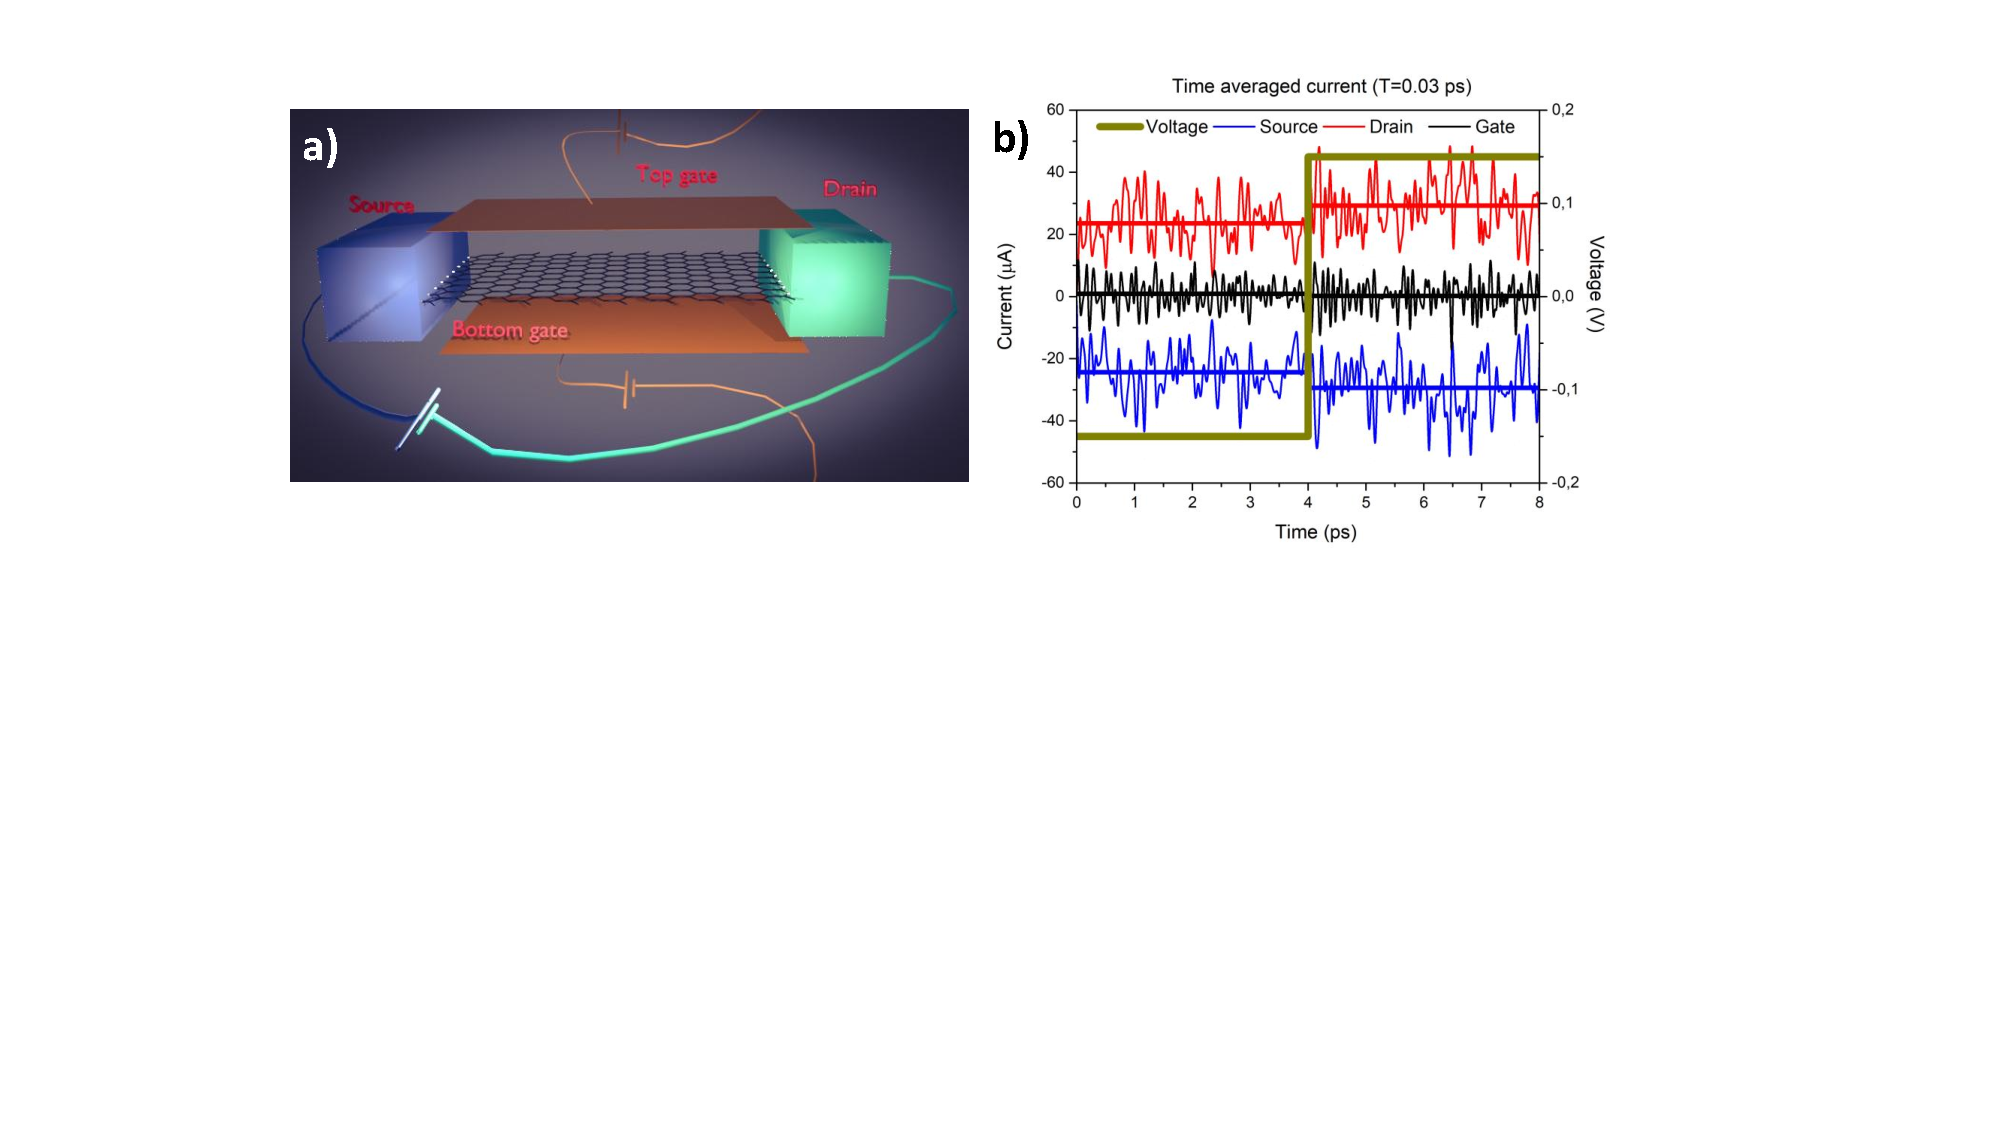
\includegraphics[width=1.05\linewidth]{Figures/figurefinal.pdf}\vspace{-0.3cm}
   \caption{(a).- Schematic representation of the FET with a graphene channel. (b) The high frequency line is the instantaneous current (time-averaged at a window of $0.03$ ps) as a function of time. The straight line is a wider averaging window of 4 ps, where we can assert the binary response.}\vspace{-0.5cm}
  \label{fig:fig}
\end{figure}


%\newpage
%\subsubsection*{2.2. Towards another general framework to look for position SSE-s}
%We have developed a second framework to look for SSE-s (equations to evolve CWF-s independently), based on the Born-Huang ansatz of the full wavefunction, at the cost of having a suitable guess for the conditional energy eigenstates of the relevant parts of the environment. For this, given the full, subsystem-environment Hamiltonian $\hat{H}(\vec{x},\vec{y},t)=\sum_{k=1}^N \frac{-\hbar^2}{2m_k}\pdv[2]{}{x_k} + U(\vec{x},\vec{y},t)+V(\vec{x},t)$,\footnote{The classical potentials $U,V$ are allowed to have explicit time dependences to account for classical interactions with the rest of the environment.} we can define the transversal section Hamiltonian as $\hat{H}_x(\vec{y},t):=\sum_{k=m+1}^N\frac{-\hbar^2}{2m_k}\pdv[2]{}{x_k}+U(\vec{x},\vec{y},t)$. Then, we define the set of eigenstates $\{\Phi^j_x(\vec{y},t)\}_j$ with eigenvalues $\{\varepsilon_x^j(t)\}_j$, parametrized by the chosen section $\vec{x}$, to be the solution of: $\hat{H}_x(\vec{y},t)\Phi^j_x(\vec{y},t)=\varepsilon_x^j(t)\Phi^j_x(\vec{y},t)$. We call these states $\Phi^j_x(\vec{y},t)$, the transversal section eigenstates (TSE). Since the hermiticity of the operator $\hat{H}_x(\vec{y},t)$ implies the TSE-s form an orthonormal basis for the Hilbert space of $\vec{y}$ at each $\vec{x}$, we could expand the following ansatz: $\Psi(\vec{x},\vec{y},t)=\sum_j \Lambda^j(\vec{x},t)\Phi_x^j(\vec{y},t)=\sum_j \varphi_j(\vec{x},\vec{y},t)$, with $\Lambda^j(\vec{x},t):=\int\Phi^j_x(\vec{y},t)\Psi(\vec{x},\vec{y},t)dy$ the projection coefficients and $\varphi_j(\vec{x},\vec{y},t):=\Lambda^j(\vec{x},t)\Phi^j_x(\vec{y},t)$.

%Now, using this expansion in the Schrödinger Equation, and evaluating the full wavefunction along the trajectory for the environment $\vec{y}=\vec{y}^{\:\xi}(t)$\footnote{In reality, we could choose any trajectory we like for the environment if we are not interested in computing Bohmian trajectories. Thus, it could be the result of a measurement of the environment, or just a set of trajectories that leads us to the reconstruction of the reduced density with the least number of them.}, we can get by denoting $\varphi^k_\xi(\vec{x},t):=\varphi^k(\vec{x},\vec{y}^{\:\xi}(t),t)$:
%\begin{equation}
% i\hbar\pdv{}{t}\varphi^k_\xi(\vec{x},t)=\qty[-\sum_{s=1}^m\frac{\hbar^2}{2m_s}\pdv[2]{}{x_s}+ \varepsilon^k(\vec{x},t)+V(\vec{x},t)   +i\hbar \dv{}{t}log(\Phi^k_x(\vec{y}^{\, \xi}(t),t))]\varphi^k_\xi(\vec{x},t)+
%\end{equation}
%$$
%\hspace{-0.4cm}+\sum_{j=0}^\infty\sum_{s=1}^m \frac{-\hbar}{2m_s}\qty( \frac{1}{\Phi^j_x(\vec{y}^{\, \xi}(t),t)}\pdv[2]{\Phi^j_x(\vec{y}^{\, \xi}(t),t)}{x_s}+2\pdv{}{x_s}log(\Phi^j_x(\vec{y}^{\, \xi}(t),t))\qty[\pdv{}{x_s}-\pdv{}{x_s}log(\Phi^j_x(\vec{y}^{\, \xi}(t),t))] )\varphi^j_\xi(\vec{x},t)
%$$
%Because the CWF for the subsystem can be recovered from $\psi^\xi(\vec{x},t)=\sum_j \varphi^j_\xi(\vec{x},t)$, we have obtained a set of {\bf exact} linear equations involving only $n$ dimensional states (instead of $N$) that allow the evolution of single CWF-s. In principle, since a general Hilbert space will need to have a countably infinite number of orthonormal states in a basis, it would be a set of infinite number of equations. However, we shall reasonably truncate the expansion of the CWF at a relatively low fixed point (at which for example the norm of the CWF surpasses a certain threshold), or even allow it to vary in time. If so, the difficulty of these equations would only relay on the knowledge of the TSE-s $\Phi^j_x(\vec{y},t)$. The point is that providing educated guesses for them seems to be more reasonable than guessing for $G$ and $J$ \eqref{G.Bohm}, \eqref{J.Bohm}. Thus, this might be the starting point for the derivation of SSE-s for a particular non-Markovian environment, which as said previously, will need to be approximate in general.  \vspace{-0.2cm}

 
\subsection*{3. When the Unspeakables Become Both Speakable and Operational}

Retaking the discussion in the beginning of the chapter, under the orthodox {\em eigenstate-eigenvalue link} we can only say a quantum system {\bf has} a defined property when its wavefunction is an eigenstate of the operator related to that property. Since a strong measurement, as we have seen, always forces the system to adopt an eigenstate, while the unitary evolution in the meantime, will cause a superposition in general, we are only allowed to speak about properties of {\bf measured} quantum systems. %However, this implies an engineer cannot talk about the electrons in the nanometric active region of a device, since if anything, it is the cables coupled to that active region that are measured. This leaves the electrons only weakly measured and thus in general, their wavefunction, in a superposition. 

This impediment poses {\bf practical} difficulties, for instance when trying to measure the maximum working frequency of nano-scale transistors to test the performance of modern computers \cite{modern}. For this, the time spent by electrons in the active region of the transistors, their {\bf dwell time}, must be measured. The eigenstate-eigenvalue link would force us to place position detectors in the two ends of the active region. However, the obtained metric would be meaningless, since in operation no computer has such detectors at the ends of its transistors \cite{tunnel1, tunnel2}; and every measurement produces a collapse backaction in the system, causing its subsequent evolution to be different than otherwise. The quantum measurement, no matter how weak it is, introduces an effective collapse backaction in the system that disrupts its future evolution, and disrupts it in a way dependent on the particular measurement scheme employed (say the ancilla fiducial state). This poses a clear impasse when looking in general, for two time information about the evolution of a closed system. An additional example happens in thermodynamics: because {\bf work} is by definition a dynamical property implying at least two times, it seems there is no possible universal definition for a quantum work operator \cite{nogo, workPb1, workPb2}. Perhaps more in general, {\bf two time correlations} of non-commuting observables, say $F$ and $B$, cannot be defined without including an explicit disturbance by a particular measurement scheme. We could correlate the result of a strong measurement of $F$ at time $t_1$ and a strong measurement of $B$ at time $t_2$, but since the measurement at $t_1$ will project the state to different EWF-s, the backaction of the measuring device will be obvious. Even numerically it seems hard to be well defined. If their operators do not commute, $\langle \hat{B}(t_2)\hat{F}(t_1)\rangle$, in the Heisenberg formalism, will give a complex number in general. We could just take the real part $\mathbb{R}e \big\{\langle \hat{B}(t_2)\hat{F}(t_1)\rangle\big\}$, which turns out to be the correlation of a weak measurement \cite{Weak} of $F$ at time $t_1$ and a strong measurement of $B$ at time $t_2$. Yet, as shown in \cite{spin}, even an ideally weak measurement does in fact perturb the system in a way that is dependent, for example, on the particular fiducial state employed for it. Then, are we fundamentally forbidden to access dynamical information about the "unmeasured system"\footnote{A system that is not being measured, e.g. a closed system evolving without quantum interaction with its environment.}? Or else, is there a way to consistently define non-{\em contextual}\footnote{Contextual means it depends and implies the environment used to convey the information to the observer.} quantum properties? Bohmian mechanics, with its ontology being persistent even when no measurement is taking place, appears to be the escape route. But is it?  \vspace{-0.15cm}

{\bf Three impasses} need to be clarified here. First: is there a (Bohmian) way in which we can meaningfully talk about "unmeasured system" properties, and even still be in accordance with orthodox phenomenology? Second: are these "unmeasured system" properties experimentally accessible? And third: can these properties be employed to operationally compute practical information, or are they mere philosophical reliefs?

\subsubsection*{3.1. Breaking Impasse 1: Speakable information of the "unmeasured" system}\vspace{-0.15cm}

Let us first clarify what is exactly the information we gain when we measure a quantum system and whether this information is about the pre-measurement/"unmeasured" system, or the post-measurement system. Consider an observable operator $\hat{B}=\sum_b b\ket{b}\bra{b}$, with $\{\ket{b}\}_b$ an orthonormal basis and $\ket{\psi}$ the wavefunction of the pre-measurement system. We have seen that measuring $B$ will lead the system to the {\bf post}-measurement state $\ket{b}$ linked with the measured $b$, which will happen with a probability $|\bra{b}\ket{\psi}|^2$ due to the {\bf pre}-measurement state. Thus, on the one hand, three things about the post-measurement system are revealed: its state $\ket{b}$, the measured value $b$, and if it was a generalized measurement, the wave-vector in which the system coupled to the measured ancilla is left by the effective collapse of the ancilla. About the {\bf pre-}measurement system, from an orthodox perspective, we can only know the probabilities $|\bra{b}\ket{\psi}|^2$. But if a "measurement", as Bell said \cite{Bell}, has the connotation of unveiling or revealing information about the ({\bf pre-}measurement) system, it seems that it would be more proper to name this process an "experiment" rather than a "measurement". For a Bohmian there is one thing more we can know about the pre-measurement system with such an experiment: if $\hat{B}$ is a function of the position operator $f(\hat{x})$, then $b$ is the post-measurement property $B$ related with the Bohmian trajectory (say, its position), and since the trajectory must be continous in time, at least it will be linked with the pre-measurement property $B$. Yet, if $\hat{B}$ does not commute with $\hat{x}$, it is not clear how the measured $b$ could be related to the "unmeasured" system. Let us clarify how the continuous ontological existence of the Bohmian trajectory can let us give any operator $\hat{B}$ a definition in terms of pre-measured system information, and with it break the "unspeakables".

Given any arbitrary (Hermitian) operator $\hat{B}$, describing the observable property $B$ for the subsystem S, with normalized EWF $\ket{\psi(t)}$, let us first blindly define the function $C^{\psi}(x,t):=\frac{\bra{\vec{x}}\hat{B}\ket{\psi(t)}}{\bra{\vec{x}}\ket{\psi(t)}}$. It seems just a cumbersome definition, yet, write the expected value for $\hat{B}$  as a function of $C^\psi(x,t)$:
\begin{equation}
\langle \hat{B}\rangle(t)= \bra{\psi(t)}\hat{B}\ket{\psi(t)}=\int \bra{\psi(t)} \ket{\vec{x}}\bra{\vec{x}}\hat{B}\ket{\psi(t)}dx =  \int |\psi(\vec{x},t)|^2C^\psi(\vec{x},t)dx
\end{equation}
This means that the spatial average of the (possibly complex) $C^\psi(\vec{x},t)$ gives at all times, the same expected value for the observable $B$ as the one given by the standard theory. Then, let us define a real function $\B^\psi(\vec{x},t):=\mathbb{R}e\{C^{\psi}(x,t)\}$. Because $\hat{B}$ is an observable, its expected value will be a real number, then: $\langle \hat{B}\rangle=\mathbb{R}e\{\langle \hat{B}\rangle\}$. Thus, the expectation could equivalently be computed as:
\begin{equation}
\langle \hat{B}\rangle(t)=\int |\psi(\vec{x},t)|^2\B^\psi(\vec{x},t)dx= \lim_{|\Sigma|\rightarrow \infty}\frac{1}{|\Sigma|} \sum_{\xi\in\Sigma} \B^\psi(\vec{x}^{\:\xi}(t),t)
\end{equation}
where we additionally used the Quantum Equilibrium hypothesis \cite{Absolute} for the set of trajectories $\{\vec{x}^{\:\xi}(t)\}_{\xi\in\Sigma}$ sampled in independent repetitions of the experiment. This equation means that the real number $\B^\psi(\vec{x}(\vec{\xi},t),t)$ related to the $\vec{\xi}$-th Bohmian trajectory, averaged over the ensemble of possible trajectories, gives the same value as the operator's expectation. This means that  irrespective of whether we give the observable $B$ an ontological status or not, we can understand $\B^\psi(\vec{x},t)$ as the feature $B$ of the Bohmian trajectory passing from $\vec{x}$ at time $t$. We will call $\B^\psi$, the "property $B$ of the Bohmian trajectory at $(\vec{x},t)$", with which we just mean for now "numerical information linked with the trajectory", meaning nothing about its ontological nor operational status.

$\B^\psi$ appears to be just an ad-hoc function of the trajectories for the operator expected value to be satisfied. But, what would this property be for each trajectory if the system state, $\ket{\psi}$, was an eigenstate of $\hat{B}$ with eigenvalue $b$?
\begin{equation}
\B^\psi(\vec{x})=\mathbb{R}e\qty{ \frac{\bra{\vec{x}}\hat{B}\ket{\psi}}{\bra{\vec{x}}\ket{\psi}} } = \mathbb{R}e\qty{ \frac{\bra{\vec{x}}\ket{\psi}b}{\bra{\vec{x}}\ket{\psi}} }=b\quad \forall \vec{x}
\end{equation}
This suggests $\ket{\psi}$ is an eigenstate of $\hat{B}$ if and only if it is a state for which every Bohmian trajectory has the same value of the property $\B^\psi$. On the one hand, this tells us that philosophically, the $b$ indicated by the dial of a projective measurement, can always be considered to be information linked to the Bohmian trajectory, even when its operator does not commute with position. On the other hand, in practice, it can be a tool to construct the operator $\hat{B}$ itself. Just define $\hat{B}$ in terms of $\B^\psi$, as the collection of states $\ket{b}$ in which all Bohmian trajectories have the same value $b$ for $\B^\psi$.

If the explicit shape of $\B^\psi$ had nothing to do with Bohmian mechanics, this reverse definition of $\hat{B}$ could be a circular definition. However, it turns out that if we set as $\hat{B}$, the momentum operator $\hat{p_k}$ of the $k$-th degree of freedom, the trajectory property $\B^\psi(\vec{x},t)$ is exactly equal to the Bohmian momentum of the trajectory crossing $\vec{x}$: $m_k v_k(\vec{x},t)$ \cite{DevInPosition1}. If we set as $\hat{B}$, the Hamiltonian operator $\hat{H}$, the property $\B^\psi(\vec{x},t)$ turns out to be exactly equal to the Bohmian energy (kinetic plus classical and quantum potentials \cite{JordiXavier}) of the trajectory crossing $\vec{x}$. And the list of these "fortunate" matches for an "ad-hoc" definition that seemed to be designed only to satisfy the expectation values, goes on. This suggests that we can employ Bohmian mechanics to derive the expression for $\B^\psi$, thanks to its similarity with classical mechanics, and then define the related operator in its terms. This is already useful theoretically, give $\B^\psi$ an ontological status or not, be it operational or not, because there are observables, like the displacement current in a nano-device, for which there is no clear operator, but there is a clear Bohmian observable associated with it, as we will see \cite{Pel, equiv}.

In a nutshell, since we placed no restriction on $\hat{B}$, we are mathematically safe to assume that at all times, each Bohmian trajectory $\vec{\xi}$, has a simultaneously determined value $\B^\psi(\vec{x}^{\:\xi}(t),t)$ linked to {\bf every} observable operator $\hat{B}$ (independently of their ontological status). Moreover, the functions $\B^\psi$ related to {\bf ontic properties}\footnote{Properties that the theory defines to be part of the ontology.} (in Bohmian mechanics) like the momentum, or some other properties like the energy, turn out to match with their Bohmian definitions, allowing us to predict operators for complicated observables using Bohmian mechanics. Then, because there is a feature $\B^\psi$ related to the Bohmian trajectories, for {\bf every} observable $\hat{B}$, and because the trajectories exist in the absence of observation in the Bohmian theory: within this theory, there is a speakable "property" $\B^\psi$, with a well defined value at all times, available for any observable. These properties $\B^\psi$ in addition evolve in time following the classical intuition.\footnote{This last has yet another striking consequence: if $b$ is the observed value for a trajectory after a von Neumann coupling (thus the value we measure strongly), and the trajectory had another value for $\B^\psi$ before the interaction started (because say, the pre-measurement state was not an eigenstate of $\hat{B}$), then the property $\B^\psi$ took all intermediate values before taking $b$, not necessarily among the eigenvalues of $\hat{B}$. Thus, if we want, we are safe to see the "quantization" of quantum mechanics as an apparent property, due to the fact that for a "proper" measurement, we require that a dial saying $b$ is compatible with a wavefunction $\ket{b}$ that will give a measurement $b$ with probability 1. That is, a wavefunction which has all its Bohmian trajectories with value $b$ for $\B^\psi$. Then, we call it "quantum" because this delicate orchestration can only happen for a certain "quantized number" of wavefunctions.}

\subsubsection*{3.2. Breaking Impasse 2: Is this "unmeasured" system information operational?}\vspace{-0.15cm}

If we could only obtain $\B^\psi$ in a laboratory when we forced it with a strong von Neumann interaction, to be an eigenvalue of $\hat{B}$, all this would limit us in practice the same way as the eigenstate-eigenvale link, even if we could now speak about the properties in the abscense of measurement. If so, we could not strictly say that $\B^\psi$ are {\bf operational properties}\footnote{Properties that can be obtained in a laboratory with a well-defined prtotocol.} of the unmeasured system. However, it turns out we can actually obtain the "unmeasured" $\B^\psi$ for any pre-measurement system and time. The "how", explains the "cumbersome" definition $\B^\psi(\vec{x},t)=\mathbb{R}e\{\bra{\vec{x}}\hat{B}\ket{\psi}/\bra{\vec{x}}\ket{\psi}\}$. It turns out to be the protocol that naive classical experimentalists \cite{WisemanVel} would follow if they thought the system had a defined position, initially uncertain to us, and the only quantum knowledge they had was that measurement interactions spoil the system's natural subsequent evolution. In order to know the property $B$ of such a subsystem S (say, an electron) when it crosses $\vec{x}$, they would first couple an ancilla A to the subsystem S of EWF $\ket{\psi}$, through the measurement Hamiltonian $\bar{\mu}(t)\,\hat{p}_A\otimes\hat{B}$ but letting the interaction strength $\mu$ be very small, such that the system state is only slightly perturbed. They would strongly measure the slightly entangled ancilla's position and get a weak measurement about the property $B$ of S. Before the slightly perturbed system S further evolved, they would strongly measure its position. Finally, they would average the weak measurements of $B$ for which the system S (the electron) was found at $\vec{x}$, in order to erase the noise introduced by the weakness of the coupling with A. It turns out, if the averaged ensemble is big enough, the resulting number will be exactly equal to $\B^\psi(\vec{x},t)$, as proved in Refs. \cite{Weak, DevInPosition1} (this is called a position post-selected weak value). A naive experimentalist, would not be surprised at all by such a "coincidence". One can consider all this was juggling with results of several observations. But, one can also perfectly legitimately say, that the average weak measurements of $B$, for experiments in which the system (the electron) was at $\vec{x}$, gave $\B^\psi(\vec{x},t)$, because whenever the Bohmian trajectory (the electron) was at $\vec{x}$, it had indeed the property $\B^\psi(\vec{x},t)$. For ontic properties, such a consideration is indeed natural. However, because we can do this protocol in theory for any observable $\hat{B}$, irrespective of its ontic state, $\B^\psi(\vec{x},t)$ is always an {\bf operational property} \cite{DevInPosition1, DevInPosition2}.\vspace{-0.15cm}


\subsubsection*{3.3. Breaking Impasse 3: Is this operational information useful for a non-Bohmian?}
\vspace{-0.15cm}

Regardless of whether one is ready to accept an ontological status for any of these $\B^\psi$ operational properties, their relation with expected values and the definition of the observable operator $\hat{B}$ is mathematically true. It is also true they are numbers describing the pre-measurement wavefunction $\ket{\psi}$, and it is true they are experimentally accessible. All this leads to practical applications, equally useful for a non-Bohmian.

On the one hand, we can numerically predict the expected value for an observable without the need to have explicitly defined its formal operator. One can derive the observable $\B^\psi(x,t)$ in the language of Bohmian mechanics and compute the ensemble average of the property to get the expected value of the operator related to it. For example, this is how we predict the total electrical current crossing the active region of a two-terminal nano-device operating at high frequencies (THz) in the BITLLES simulator \cite{equiv, Pel}. The total current at such frequencies needs to consider the displacement component. We can define the current due to the Bohmian trajectory of a $k$-th electron $\vec{x}_k^{\:\xi}(t)$ of charge $e$ through a surface $\sigma$ as: $I_k^{(\xi)}(t)=\int_\sigma \vec{J}^{\:(\xi)}(\vec{r},t)\cdot d\vec{s}+\int_\sigma \varepsilon(\vec{r},t)\pdv{\vec{E}^{\:(\xi)}(\vec{r},t)}{t}\cdot d\vec{s}$, where $\varepsilon(\vec{r},t)$ is the electric permittivity , $\vec{J}^{\:(\xi)}(\vec{r},t)=e\dv{\vec{x}_k^{\:\xi}(t)}{t}\delta(\vec{r}-\vec{x}_k^{\:\xi}(t))$ is the particle current density, and $\vec{E}^{\:(\xi)}(\vec{r},t)$ is the electric field generated by the electron, as a solution to the Gauss equation.\footnote{The legitimacy of a well defined electric field in Bohmian mechanics is proven for example in \cite{lightMatter}.} Then, as proven in \cite{Pel}, for two terminal devices of longitudinal length $L$, with metallic contact surfaces $\sigma$, of width and height $w,h>>L$, the total current contribution in these surfaces is: $I^{(\xi)}_k(t)=\frac{e}{L}v_x^{(\xi)}(\vec{x}=\vec{x}_k^{\:\xi}(t), t) $, where $v_x$ is the longitudinal Bohmian velocity of the electron. The total Bohmian current at the surface $\sigma$ will then be the sum of these contributions $I^{(\xi)}(t)=\sum_k I^{(\xi)}_k(t)$, such that we can get the phenomenological expectation of the operator $\hat{I}$, by a simple ensemble average: $\mathbb{E}_\xi [I^{(\xi)}(t)]=\langle \hat{I}\rangle(t)$. 


On the other hand, these operational properties provide a practical answer to the search of non-contextuality in the dynamical variables involving two different times \cite{DevInPosition1}. 

{\bf (1.)} The problem of non-contextual two-time correlations of dynamical variables for a wavefunction $\ket{\psi(t)}$, can be circumvented by computing the expectation as would be done by a frequentist definition in a classical system. Given a big enough set of trajectories $\{\vec{x}^{\:\xi}(t)\}_{\xi\in \Sigma}$ each with associated properties $\B^\psi(\vec{x},t)$ and $\mathcal{F}^\psi(\vec{x},t)$, following quantum equilibrium \cite{Absolute} we could define:\vspace{-0.2cm}
\begin{equation}
\langle B(t_2)F(t_1)\rangle := \lim_{|\Sigma|\rightarrow \infty}\frac{1}{|\Sigma|} \sum_{\xi\in\Sigma} \B^\psi(\vec{x}^{\:\xi}(t_2),t_2)\mathcal{F}^\psi(\vec{x}^{\:\xi}(t_1),t_1) =
\end{equation}
$$
=  \int |\psi(\vec{\xi},0)|^2\ \mathbb{R}e\qty[ \frac{\bra{\vec{x}^{\:\xi}(t_2)}\hat{B}\ket{\psi(t_2)}}{\bra{\vec{x}^{\:\xi}(t_2)}\ket{\psi(t_2)}} ] \mathbb{R}e\qty[ \frac{\bra{\vec{x}^{\:\xi}(t_1)}\hat{F}\ket{\psi(t_1)}}{\bra{\vec{x}^{\:\xi}(t_1)}\ket{\psi(t_1)}} ]d\xi
$$
{\bf (2.) } In a similar way, we can solve the problems concerning a quantum work definition, just as done by \cite{work1, work2}. First note that given a general system Hamiltonian $\hat{H}=\sum_k \frac{-\hbar^2}{2m_k}\pdv[2]{}{x_k}+V(\vec{x},t)$, we get:
\begin{equation}
\mathcal{H}^\psi(\vec{x}^{\:\xi}(t),t) := \mathbb{R}e\qty[ \frac{\bra{\vec{x}^{\:\xi}(t)}\hat{H}\ket{\psi(t)}}{\bra{\vec{x}^{\:\xi}(t)}\ket{\psi(t)}} ] = \sum_{k=1}^n\frac{1}{2}m_kv_k(\vec{x}^{\:\xi}(t),t)^2+V(\vec{x}^{\:\xi}(t),t)+Q(\vec{x}^{\:\xi}(t),t)
\end{equation}
with $Q$ the well known Bohmian quantum potential \cite{Holland, Durr, JordiXavier}. This proves $\mathcal{H}^\psi(\vec{x}^{\:\xi}(t),t)$ is, as anticipated, the total Bohmian energy of the $\vec{\xi}$-th trajectory at time $t$. Then, following classical mechanics, we can compute its associated Bohmian work as the energy difference (if conservative, else employing an integral): $\mathcal{W}^{(\xi)}(t_1,t_2)= \mathcal{H}^\psi(\vec{x}^{\:\xi}(t_2),t_2)-\mathcal{H}^\psi(\vec{x}^{\:\xi}(t_1),t_1)$. As a result, a well-defined non-contextual definition of the quantum work could be the ensemble average of the trajectory works:
\begin{equation}
\langle W(t_1,t_2)\rangle = \lim_{|\Sigma|\rightarrow \infty}\frac{1}{|\Sigma|} \sum_{\xi\in\Sigma} \qty(\mathcal{H}^\psi(\vec{x}^{\:\xi}(t_2),t_2)-\mathcal{H}^\psi(\vec{x}^{\:\xi}(t_1),t_1))
\end{equation}
{\bf (3.) }Finally, we could give a reasonable Bohmian answer to the search of an "unmeasured" dwell time, as the expected time spent by the Bohmian trajectory of the electron within the active region $\Gamma\subset \R^3$. Mathematically, the dwell time $\tau$ for the $\vec{\xi}$-th trajectory of the $k$-th electron with EWF $\psi^\xi(\vec{x}_k,t)$ is by definition given by the Lebesgue integral: $\tau^{( \xi)}= \int_{0}^\infty  dt \int_\Gamma \delta(\vec{r}-\vec{x}_k^{\:\xi}(t)) dr$. This makes the expected time $\langle \tau\rangle$ be, by the quantum equilibrium hypothesis:\vspace{-0.15cm}
\begin{equation}
\langle \tau \rangle = \lim_{|\Sigma|\rightarrow \infty}\frac{1}{|\Sigma|} \sum_{\xi\in\Sigma} \tau^{(\xi)} = \int_{0}^\infty dt \int_\Gamma |\psi^\xi(\vec{r},t)|^2dr\vspace{-0.15cm}
\end{equation}
which turns out, is a well-known equation used to predict the dwell time.\vspace{-0.2cm}


\subsection*{4. Final Remarks and Conclusions}\vspace{-0.15cm}

Thus, we have seen that inherently Bohmian concepts like the conditional wavefunction or position post-selected weak values are indeed usable pragamtically as practical tools in the computation of phenomenologically accessible elements like the reduced density matrix, expectation values or time correlations. Not only that, but we have also seen with several examples that additionally dressing them with the Bohmian interpretation makes these tools even more practical, by aiding in the search of SSE-s or observable operators. But then, if we can use Bohmian concepts as a tool, why not include them in our vocabulary? The purely phenomenological orthodox view, which forbidds us to say there are electrons in the transistors of our phones, has an alternative that is operationally useful, but which can also provide us ontological relief. Why just use it to untie our hands and not also our words? Especially in a time when no engineer is really capable to accept the "unspeakeble" quantum reality \cite{where}, and when we know that not even great parents of the quantum theory were ready to restrict themselves to the Copenhagen doctrine. For example, regarding the first section, von Neumann in his seminal book \cite{vonNeumann} explains that the collpase law is to be understood as an effective process that should be possible to be placed at an arbitrary point between the subsystem and the macroscopic device, instead of considering it to be a physical phenomenon \cite{NeumannNoCollapse}. Linking this with the discussion on the contextuality of the quantum measurement that avoids a simple elucidation of the pre-measurement system, Bohr himself did not either believe in a physical collapse and instead owned it to the contextuality of experimental protocols \cite{Dirac} in terms of macroscopic devices \cite{Bohr}. The claims of both scientists are naturally satisfied by the Bohmian description of the measurement, as we reviewed, which does not need to postulate any collapse law. When it comes to the second section, it was H. M. Wiseman who pointed out that SSE-s for non Markovian systems implied the usage of CWF-s of modal theories \cite{interpretSSE, NMisModal} and who suggested the first formal position SSE-s for such open quantum systems \cite{WisemanSSE}. Finally, regarding the discussion on the unspeakables of the third section, Dirac himself was an exemplary physicist that employed "unspeakable unmeasured" system properties in the formulation of his major contributions to physics \cite{Dirac}.

With all, we might be wondering when will we decide to end up with the limiting walls around (non-relativistic) quantum mechanics, which are voluntarily taught to new generations of physicists every day. Now that there is a coherent and pedagogical narrative (the Bohmian one) to explain it all avoiding paradoxes and disjunctives with classical intuitions, a narrative that actually proves to be practically useful by offering additional tools to the standard theory. Will we someday include them in the standard quantum framework? Time will tell, because apparently common sense will not.


\newpage
\begin{thebibliography}{1}
{\footnotesize 

\bibitem{where}
Oriols X. and Ferry D. K., {\em "Why engineers are right to avoid the quantum reality offered by the orthodox theory? [point of view],"} Proceedings of the IEEE, vol. 109, no. 6, pp. 955-961, 2021.

\bibitem{Bohm}
Bohm, D. {\em "A suggested interpretation of the quanta theory in term of hidden variables: Part I."} Phys. Rev. 85, 166–179 (1952).

\bibitem{Holland}
P. R. Holland, {\em "The Quantum Theory of Motion: An account of the de Broglie-Bohm Causal Interpretation of Quantum
mechanics,"} Cambridge University Press, Cambridge 1993.

\bibitem{Durr}
Dürr D., Teufel. S. {\em "Bohmian mechanics: the physics and mathematics of quantum theory,"} Springer Science \& Business Media, Berlin, Germany, 2009.

\bibitem{JordiXavier}
	Oriols X., Mompart J., {\em "Applied Bohmian Mechanics: From Nanoscale Systems to Cosmology,"} Pan Stanford, Singapore, 2012.
	
\bibitem{Thz}
Pandey, D., Colomés, E., Albareda, G. \& Oriols, X. {\em "Stochastic Schrödinger equations and conditional states: A general non-Markovian quantum electron transport simulator for THz electronics."} Entropy 21(12), 1148 (2019).

\bibitem{Absolute}
Dürr, D., Goldstein, S. \& Zanghí, N. {\em "Quantum equilibrium and the origin of absolute uncertainty."} J Stat Phys 67, 843–907 (1992).

\bibitem{GJ}
Oriols X. {\em Quantum-trajectory approach to time-dependent transport in mesoscopic systems with electron-electron interactions} Phys. Rev. Lett. 98 066803 (2007).

%\bibitem{XOPhysSpace}
%Norsen, T., Marian, D. \& Oriols, X. {\em Can the wave function in configuration space be replaced by single-particle wave functions in physical space?.} Synthese 192, 3125–3151 (2015).

\bibitem{vonNeumann}
von Neumann, J. {\em "Mathematische Grundlagen der Quantenmechanik."} Springer Verlag, Berlin (1932).

\bibitem{NeumannNoCollapse}
Becker, Lon. {\em “That von Neumann Did Not Believe in a Physical Collapse.”} The British Journal for the Philosophy of Science 55, no. 1 (2004): 121–35.

\bibitem{Dirac}
Oldofredi, A. and Esfeld, M. (2019) {\em "Observability, Unobservability and the Copenhagen Interpretation in Dirac's Methodology of Physics."} Quanta, 8 (1). pp. 68-87.

\bibitem{Bohr}
N. Bohr. {"Essays 1932-1957 on Atomic Physics and Human Knowledge."} p.39. Wiley, New York, 1958.

%\bibitem{XOCM}
%Oriols, X., \& Benseny, A. {\em "Conditions for the classicality of the center of mass of many-particle quantum states."} New Journal of Physics, 19(6), [063031],  (2017).

\bibitem{Generalized}
Wiseman, Howard M., and Gerard J. Milburn. {\em "Quantum measurement and control."} Cambridge university press, 2009.

\bibitem{density}
Dürr, D., Goldstein, S., Tumulka, R., and Zanghí, N. {\em "On the role of density matrices in Bohmian mechanics."} Foundations of Physics 35.3 (2005): 449-467.

\bibitem{GNSTheorem}
J. B. Conway, {\em "A course in functional analysis,"} 2nd edn, Springer, New York, 1990.

\bibitem{continousMeas}
Jacobs, Kurt, and Daniel A. Steck. {\em "A straightforward introduction to continuous quantum measurement."} Contemporary Physics 47.5 (2006): 279-303.

\bibitem{MarkovianityDefs}
Li, Li, Michael JW Hall, and Howard M. Wiseman. {\em "Concepts of quantum non-Markovianity: A hierarchy."} Physics Reports 759 (2018): 1-51.

\bibitem{QuantumTrajs}
Wiseman, Howard M. {\em "Quantum trajectories and quantum measurement theory."} Quantum and Semiclassical Optics: Journal of the European Optical Society Part B 8.1 (1996): 205.

\bibitem{interpretSSE}
Gambetta, Jay, and H. M. Wiseman. {\em "Interpretation of non-Markovian stochastic Schrödinger equations as a hidden-variable theory."} Physical Review A 68.6 (2003): 062104.

\bibitem{NMisModal}
Wiseman, H. M. \& Gambetta, J. M. {\em "Pure-state quantum trajectories for general non-Markovian systems do not exist."} Phys. Rev. Lett. 101, 140401 (2008).

\bibitem{Diosi}
Diósi, Lajos, and Walter T. Strunz. {\em "The non-Markovian stochastic Schrödinger equation for open systems."} Physics Letters A 235.6 (1997): 569-573.

\bibitem{WisemanSSE}
Gambetta, Jay M., and Howard M. Wiseman. {\em "A non-Markovian stochastic Schrödinger equation developed from a hidden variable interpretation."} Fluctuations and Noise in Photonics and Quantum Optics. Vol. 5111. International Society for Optics and Photonics, 2003.

\bibitem{tdp}
Albareda, G., H. López, X. Cartoixa, J. Suné, and X. Oriols. {\em "Time-dependent boundary conditions with lead-sample Coulomb correlations: Application to classical and quantum nanoscale electron device simulators."} Physical Review B 82, no. 8 (2010): 085301.

\bibitem{Pois}
Albareda, G., J. Suné, and X. Oriols. {\em "Many-particle hamiltonian for open systems with full coulomb interaction: Application to classical and quantum time-dependent simulations of nanoscale electron devices."} Physical Review B 79.7 (2009): 075315.

\bibitem{inject}
Zhan, Zhen, et al. {\em "Time-dependent quantum Monte Carlo simulation of electron devices with two-dimensional Dirac materials: A genuine terahertz signature for graphene."} Physical Review B 99.15 (2019): 155412.

\bibitem{boundary1}
López, Hender, et al. {\em "Boundary conditions with Pauli exclusion and charge neutrality: application to the Monte Carlo simulation of ballistic nanoscale devices."} Journal of computational Electronics 7.3 (2008): 213-216.

\bibitem{boundary2}
Albareda, G., J. Suné, and X. Oriols. {\em "Many-particle hamiltonian for open systems with full coulomb interaction: Application to classical and quantum time-dependent simulations of nanoscale electron devices."} Physical Review B 79.7 (2009): 075315.

\bibitem{eph}
Colomés, E., Z. Zhan, D. Marian, and X. Oriols. {\em "Quantum dissipation with conditional wave functions: Application to the realistic simulation of nanoscale electron devices."} Physical Review B 96, no. 7 (2017): 075135.

\bibitem{diver1}
Eisenberg, B., X. Oriols, and D. Ferry. {\em "Dynamics of current, charge and mass."} Computational and Mathematical Biophysics 5.1 (2017): 78-115.

\bibitem{diver2}
Oriols, X., and D. K. Ferry. {\em "Quantum transport beyond DC."} Journal of Computational Electronics 12.3 (2013): 317-330.

\bibitem{equiv}
Marian, D., N. Zanghì, and X. Oriols. {\em "Weak values from displacement currents in multiterminal electron devices."} Physical review letters 116.11 (2016): 110404.

\bibitem{Pel}
Albareda, G., F. L. Traversa, A. Benali, and X. Oriols. {\em "Computation of quantum electrical currents through the Ramo–Shockley–Pellegrini theorem with trajectories."} Fluctuation and Noise Letters 11, no. 03 (2012): 1242008.

\bibitem{neg}
Pandey, Devashish, et al. {\em "A proposal for evading the measurement uncertainty in classical and quantum computing: Application to a resonant tunneling diode and a mach-zehnder interferometer."} Applied Sciences 9.11 (2019): 2300.

\bibitem{Bell}
J. S. Bell, {\em "Against Measurement."} Physics World 3, 33 (1990).

\bibitem{WisemanVel}
Wiseman, H. M. {\em "Grounding Bohmian mechanics in weak values and bayesianism."} New Journal of Physics 9.6 (2007): 165.

\bibitem{Weak}
Aharonov, Yakir, David Z. Albert, and Lev Vaidman. {\em "How the result of a measurement of a component of the spin of a spin-1/2 particle can turn out to be 100."} Physical review letters 60.14 (1988): 1351.

\bibitem{DevInPosition1}
Pandey, Devashish, et al. {\em "Unmeasured Bohmian properties and their measurement through local-in-position weak values for assessing non-contextual quantum dynamics."} (2019).

\bibitem{DevInPosition2}
Pandey, Devashish, et al. {\em "Identifying weak values with intrinsic dynamical properties in modal theories."} Physical Review A 103.5 (2021): 052219.

\bibitem{spin}
Pandey, Devashish, et al. Supplemental Material. {\em "Identifying weak values with intrinsic dynamical properties in modal theories."} Physical Review A 103.5 (2021): 052219.

\bibitem{nogo}
Perarnau-Llobet, M., E. Bäumer, K.V. Hovhannisyan, M. Huber and A. Acin,{\em "No-go theorem for the characterization of work fluctuations in coherent quantum systems."} Physical review letters 118, no. 7 (2017): 070601.

\bibitem{workPb1}
J. M. G. Vilar and J. M. Rubi, {\em "Failure of the Work-Hamiltonian Connection for Free-Energy Calculations." }Phys. Rev. Lett. 100, 020601 (2008).

\bibitem{workPb2}
W. Niedenzu, M. Huber, and E. Boukobza, {\em "Concepts of work in autonomous quantum heat engines."} Quantum 3, 195 (2019).

\bibitem{modern}
Z. Zhan, E. Colomés, and X. Oriols, {\em  "Limitations of the Intrinsic Cutoff Frequency to Correctly Quantify the Speed of Nanoscale Transistors."} IEEE Trans. Electron Devices 64, 2617 (2017).

\bibitem{tunnel1}
G. Orlando, C. R. McDonald, N. H. Protik, G. Vampa, and T. Brabec, {\em "Tunnelling time, what does it mean?"} J. Phys. B: At., Mol. Opt. Phys. 47, 204002 (2014).

\bibitem{tunnel2}
E. H. Hauge and J. A. Støvneng, {\em "Tunneling times: a critical review."} Rev. Mod. Phys. 61, 917 (1989).

\bibitem{work1}
D. H. Kobe, {\em "Quantum power in de Broglie–Bohm theory."} J. Phys. A: Math. Theor. 40, 5155 (2007).

\bibitem{work2}
R. Sampaio, S. Suomela, T. Ala-Nissila, J. Anders, and T. G. Philbin, {\em "Quantum work in the Bohmian framework."} Phys. Rev. A 97, 012131 (2018).

\bibitem{lightMatter}
Villani M. et al. Destefani C. F., Cartoixà X., Feiginov M., Oriols X. {\em "THz displacement current in tunneling devices with coherent electron-photon
interaction."}

}

\end{thebibliography}

\newpage
\twocolumn
\begin{thebibliography}{1}
{\footnotesize 

\bibitem{where}
Oriols X. and Ferry D. K., Proceedings of the IEEE, vol. 109, no. 6, pp. 955-961, 2021.

\bibitem{Bohm}
Bohm, D., Phys. Rev. 85, 166–179 (1952).

\bibitem{Holland}
P. R. Holland, {\em "The Quantum Theory of Motion."} Cambridge University Press, Cambridge 1993.

\bibitem{Durr}
Dürr D., Teufel. S. {\em "Bohmian mechanics: the physics and mathematics of quantum theory,"} Springer Science \& Business Media, Berlin, Germany, 2009.

\bibitem{JordiXavier}
	Oriols X., Mompart J., {\em "Applied Bohmian Mechanics: From Nanoscale Systems to Cosmology,"} Pan Stanford, Singapore, 2012.
	
\bibitem{Thz}
Pandey, D., Colomés, E., Albareda, G. \& Oriols, X., Entropy 21(12), 1148 (2019).

\bibitem{Absolute}
Dürr, D., Goldstein, S. \& Zanghí, N., J Stat Phys 67, 843–907 (1992).

\bibitem{GJ}
Oriols X., Phys. Rev. Lett. 98 066803 (2007).

%\bibitem{XOPhysSpace}
%Norsen, T., Marian, D. \& Oriols, X. {\em Can the wave function in configuration space be replaced by single-particle wave functions in physical space?.} Synthese 192, 3125–3151 (2015).

\bibitem{vonNeumann}
von Neumann, J. {\em "Mathematische Grundlagen der Quantenmechanik."} Springer Verlag, Berlin (1932).

\bibitem{NeumannNoCollapse}
Becker, Lon. The British Journal for the Philosophy of Science 55, no. 1 (2004): 121–35.

\bibitem{Dirac}
Oldofredi, A. and Esfeld, M. (2019). Quanta, 8 (1). pp. 68-87.

\bibitem{Bohr}
N. Bohr. {"Essays 1932-1957 on Atomic Physics and Human Knowledge."} p.39. Wiley, New York, 1958.
%\bibitem{XOCM}
%Oriols, X., \& Benseny, A. {\em "Conditions for the classicality of the center of mass of many-particle quantum states."} New Journal of Physics, 19(6), [063031],  (2017).

\bibitem{Generalized}
Wiseman, Howard M., and Gerard J. Milburn. {\em "Quantum measurement and control."} Cambridge university press, 2009.

\bibitem{density}
Dürr, D., Goldstein, S., Tumulka, R., and Zanghí, N. Foundations of Physics 35.3 (2005): 449-467.

\bibitem{GNSTheorem}
J. B. Conway, {\em "A course in functional analysis,"} 2nd edn, Springer, New York, 1990.

\bibitem{continousMeas}
Jacobs, Kurt, and Daniel A. Steck. Contemporary Physics 47.5 (2006): 279-303.

\bibitem{MarkovianityDefs}
Li, Li, Michael JW Hall, and Howard M. Wiseman. Physics Reports 759 (2018): 1-51.

\bibitem{QuantumTrajs}
Wiseman, H. M., Quantum and Semiclassical Optics: J. Eur. Opt. Soc. Part B 8.1 (1996): 205.

\bibitem{interpretSSE}
Gambetta, Jay, and H. M. Wiseman. Phys. Rev. A 68.6 (2003): 062104.

\bibitem{NMisModal}
Wiseman, H. M. \& Gambetta, J. M. Phys. Rev. Lett. 101, 140401 (2008).

\bibitem{Diosi}
Diósi, Lajos, and Walter T. Strunz. Physics Letters A 235.6 (1997): 569-573.

\bibitem{WisemanSSE}
Gambetta, J. M., and H. M. Wiseman. Fluctuations and Noise in Photonics and Quantum Optics. Vol. 5111. International Society for Optics and Photonics, 2003.

\bibitem{tdp}
Albareda, G., H. López, X. Cartoixa, J. Suné, and X. Oriols. Phys. Rev. B 82, no. 8 (2010): 085301.

\bibitem{Pois}
Albareda, G., J. Suné, and X. Oriols. Phys. Rev. B 79.7 (2009): 075315.

\bibitem{inject}
Zhan, Zhen, et al. Phys. Rev. B 99.15 (2019): 155412.

\bibitem{boundary1}
López, Hender, et al. Journal of computational Electronics 7.3 (2008): 213-216.

\bibitem{boundary2}
Albareda, G., J. Suné, and X. Oriols. Phys. Rev. B 79.7 (2009): 075315.

\bibitem{eph}
Colomés, E., Z. Zhan, D. Marian, and X. Oriols. Phys. Rev. B 96, no. 7 (2017): 075135.

\bibitem{diver1}
Eisenberg, B., X. Oriols, and D. Ferry. Computational and Mathematical Biophysics 5.1 (2017): 78-115.

\bibitem{diver2}
Oriols, X., and D. K. Ferry. Journal of Computational Electronics 12.3 (2013): 317-330.

\bibitem{equiv}
Marian, D., N. Zanghì, and X. Oriols. Physical review letters 116.11 (2016): 110404.

\bibitem{Pel}
Albareda, G. et al. Fluctuation and Noise Letters 11, no. 03 (2012): 1242008.

\bibitem{neg}
Pandey, D., et al. Applied Sciences 9.11 (2019): 2300.

\bibitem{Bell}
J. S. Bell, Physics World 3, 33 (1990).

\bibitem{WisemanVel}
Wiseman, H. M. New Journal of Physics 9.6 (2007): 165.

\bibitem{Weak}
Aharonov, Yakir, David Z. Albert, and Lev Vaidman. Physical review letters 60.14 (1988): 1351.

\bibitem{DevInPosition1}
Pandey, D., et al. (2019). https://pure.mpg.de/rest/\\ items/item\_3179219/component/file\_3179220/content

\bibitem{DevInPosition2}
Pandey, Devashish, et al. Phys. Rev. A 103.5 (2021): 052219.

\bibitem{spin}
Pandey, Devashish, et al. Supplemental Material. Phys. Rev. A 103.5 (2021): 052219.

\bibitem{nogo}
Perarnau-Llobet, M., E. Bäumer, K.V. Hovhannisyan, M. Huber and A. Acin, Physical review letters 118, no. 7 (2017): 070601.

\bibitem{workPb1}
J. M. G. Vilar and J. M. Rubi, Phys. Rev. Lett. 100, 020601 (2008).

\bibitem{workPb2}
W. Niedenzu, M. Huber, and E. Boukobza, Quantum 3, 195 (2019).

\bibitem{modern}
Z. Zhan, E. Colomés, and X. Oriols, IEEE Trans. Electron Devices 64, 2617 (2017).

\bibitem{tunnel1}
G. Orlando, et al. J. Phys. B: At., Mol. Opt. Phys. 47, 204002 (2014).

\bibitem{tunnel2}
E. H. Hauge and J. A. Støvneng, Rev. Mod. Phys. 61, 917 (1989).

\bibitem{work1}
D. H. Kobe, J. Phys. A: Math. Theor. 40, 5155 (2007).

\bibitem{work2}
R. Sampaio, S. Suomela, T. Ala-Nissila, J. Anders, and T. G. Philbin, Phys. Rev. A 97, 012131 (2018).

\bibitem{lightMatter}
Villani M. et al. {\em "THz displacement current in tunneling devices with coherent electron-photon
interaction."}

}
\end{thebibliography}

\end{document}






